\documentclass[11pt,letterpaper]{article}
\usepackage[left=0.91in,right=0.91in,top=0.92in,bottom=0.95in,headheight=14pt,headsep=15pt]{geometry}
\usepackage{fontspec}
\usepackage{libertinus}
\usepackage{microtype,graphicx,amsmath,array,booktabs,xltabular}
\usepackage{caption}
\usepackage[section]{placeins}
\usepackage{titlesec,enumitem,fancyhdr}
\usepackage[dvipsnames]{xcolor}
\definecolor{ink}{HTML}{253044}
\definecolor{accent}{HTML}{43537C}
\usepackage[unicode,colorlinks=true,urlcolor=accent,linkcolor=accent]{hyperref}
\hypersetup{pdftitle={From Published Evidence to Analyzable Biomedical Cohorts with Scientific Agents}, pdfauthor={}}
\setcounter{secnumdepth}{2}
\titleformat{\section}{\sffamily\Large\bfseries\color{ink}}{\thesection}{.65em}{}
\titleformat{\subsection}{\sffamily\large\bfseries\color{ink}}{\thesubsection}{.65em}{}
\titlespacing*{\section}{0pt}{2.2ex plus .4ex minus .1ex}{.9ex}
\titlespacing*{\subsection}{0pt}{1.7ex plus .3ex minus .1ex}{.6ex}
\captionsetup{font=small,labelfont={bf,color=ink},labelsep=period,justification=raggedright,singlelinecheck=false}
\setlength{\parindent}{0pt}
\setlength{\parskip}{.45em plus .08em minus .03em}
\setlength{\LTpre}{.9em}
\setlength{\LTpost}{.9em}
\setlength{\LTcapwidth}{\textwidth}
\setlength{\textfloatsep}{16pt plus 4pt minus 2pt}
\setlength{\intextsep}{12pt plus 3pt minus 1pt}
\setcounter{topnumber}{3}
\renewcommand\topfraction{.85}
\renewcommand\bottomfraction{.7}
\renewcommand\textfraction{.12}
\renewcommand\floatpagefraction{.68}
\renewenvironment{abstract}{\small\par\noindent{\sffamily\bfseries\color{ink}Abstract}\quad\ignorespaces}{\par\medskip}
\pagestyle{fancy}
\fancyhf{}
\fancyhead[L]{\small\sffamily\color{accent}Evidence-guided virtual cohorts}
\fancyhead[R]{\small\sffamily\color{accent}Methods development draft}
\fancyfoot[R]{\small\sffamily\thepage}
\renewcommand\headrulewidth{0.25pt}
\raggedbottom
\emergencystretch=1em
\begin{document}
\thispagestyle{plain}
{\sffamily\footnotesize\color{accent}\bfseries METHODS DEVELOPMENT DRAFT\quad\textbar\quad NOVEMBER 2026\par}
\vspace{.7em}
{\raggedright\sffamily\bfseries\fontsize{24}{29}\selectfont\color{ink}From Published Evidence to Analyzable Biomedical Cohorts with Scientific Agents\par}
\vspace{.5em}
{\small Author and affiliation details pending confirmation\par}
\vspace{.7em}
\begin{abstract}

Biomedical studies often make aggregate findings available while the individual measurements needed for a new analysis remain inaccessible. We study whether a scientific agent can turn such evidence and a research request into analyzable virtual cohorts. Within a host-reviewed workflow, the agent interprets study conditions, chooses a joint stochastic model, and supplies numerical relationships and explicit assumptions; statistical tools execute the model and inspect its outputs. In a developmental open-retrieval evaluation on previously exposed project references, four constructions produced twelve complete cohorts. All six requested glycemia analyses retained their sample-reference point directions across draws, with differing magnitude agreement; both constructions for one population preserved attenuation of the BMI coefficient after glucose adjustment. In a separate developmental two-case experiment with twenty agent constructions, the arms given additional published relationship evidence had smaller mean absolute discrepancy for five of six regression coefficients. Comparisons with a fixed statistical completion favored the agent arm in four of six relationship-evidence analyses. Iron-status and lipid results showed selected agreements alongside substantial joint-dependence and dispersion mismatches; the sealed iron comparison disagreed on its primary odds ratio, and an earlier prospective evaluation failed both overall criteria. These findings demonstrate evidence-to-model construction and partial agreement on specified analyses without target individual-level training records. Reliable inference for a new population remains unestablished.

\end{abstract}

\section{Introduction}

A researcher wants to analyze how BMI, age and glucose relate to HbA1c in a population for which individual measurements are unavailable. Published studies provide pieces of the required information: biomarker summaries, age profiles and regressions adjusted for different covariates. These findings do not arrive as a joint dataset or a complete simulation model. To run a multivariable analysis, someone must decide how the pieces can be combined and which additional relationships must be assumed.


We study an evidence-to-data workflow in which a scientific agent undertakes that modeling work. The researcher specifies the population, measurements and intended analyses. The agent works from reviewed evidence or retrieves studies under the task's access rules, chooses how to connect the variables, and authors a stochastic generator. Its output is a virtual cohort accompanied by the executable model and a record of source-supported and assumed choices. Researchers can then apply ordinary regression, stratified or other specified analyses to its records. Complete generation requires no target individual-level training records; optional observed variables can instead support enrichment or partial completion.


The research question is whether the resulting data preserve the information needed for the requested analyses. A single coefficient is not enough to describe this property. The same cohort may need to support both a BMI regression adjusted for age and sex and a second regression additionally adjusted for glucose. Agreement requires a useful joint construction, while the source studies may report only separate projections. An agent can choose such a construction, but the assumptions it adds can also produce biased effects, weak interactions or insufficient individual variation.


Our contribution is an implemented scientific-agent procedure for authoring joint biomarker models from incomplete, heterogeneous published evidence, together with an empirical evaluation of requested scientific analyses on the resulting records. The agent interprets source populations, measurement scales and adjustment sets, chooses a joint sampling law, and records its numerical evidence and assumptions. Repeated glycemia constructions and a comparison with and without additional relationship evidence assess coefficient agreement and adjustment behavior; iron-status and lipid analyses show how selected agreements coexist with errors in joint dependence, dispersion and population transfer. Published-model reconstruction and earlier prospective tests retain separate roles. This study characterizes the capabilities and limits of agent-authored biomedical model construction for specified analyses.


\section{Related work and problem definition}

\subsection{From available information to analyzable records}

Filshtein et al. share fitted study models so a recipient can simulate complete cohorts for epidemiological analyses [1]. SynthIPD uses published survival curves and trial summaries to reconstruct time-to-event records with covariates [2]. SynDI combines internal individual data with external regression information across populations to fit a target regression [29]. Multilevel network meta-regression likewise relates aggregate evidence to individual-level models under population assumptions [3]. These approaches differ in what the recipient knows. Filshtein et al. supply the comparison for our HRS experiment because the published exports and the scientific analysis can be matched. In our external-evidence experiments, the agent must also choose the joint dependence structure needed to perform the requested analyses.


G-Sim combines LLM-authored simulators with numerical calibration and structural refinement [4]. LLMSynthor infers relevant variable dependencies and uses aggregate discrepancies to guide proposals for new records, with evaluations of downstream predictive utility and household population queries [5]. SynthCraft studies healthcare synthetic-data workflows [6], and SPADA samples from a dependency graph fitted with observed tabular data [15].


KMGen combines agentic extraction of published Kaplan–\allowbreak{}Meier curves and trial information with explicit clinical priors and a specified mechanistic sampler to generate patient survival and adverse-event records [36]. Jones et al. generate household populations from aggregate demographics without individual input data, use statistical feedback and examine household relationships not supplied as constraints [37,38]. These studies already connect language models, published or aggregate evidence and synthetic records. Our experiments examine how an agent authors joint biomarker models for different research requests, handling source populations, measurement scales and adjustment sets, and which scientific analyses their records support. They do not establish quality or scaling superiority over these systems.


\subsection{System architecture}

Figure 1 centers on the decision that changes the data. A scientific agent proposes a joint model, writes a program to sample it, and records which parts follow from published evidence and which it supplied. A numerical worker executes a trial of that program. The coordinator returns the checks allowed by the study. The agent can keep the model or revise it within the study budget. The output is a versioned generator and a cohort that other researchers can analyze.


\begin{figure}[htbp]

\centering

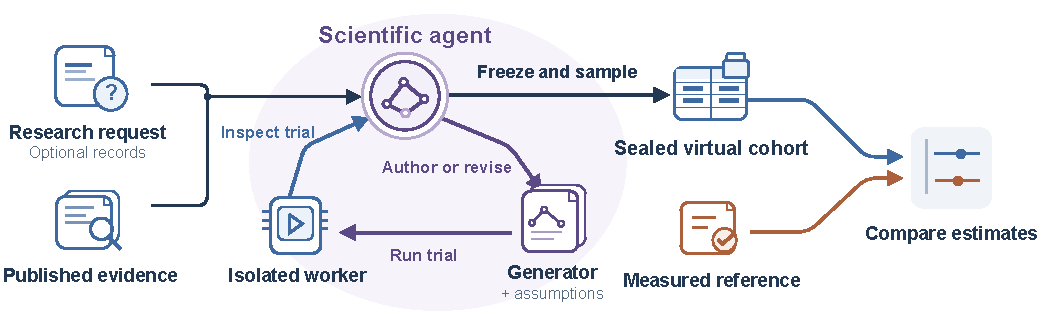
\includegraphics[width=\linewidth]{figures/fig1-agent-loop.drawio.pdf}

\caption{The scientific agent's action and feedback loop. The agent authors a generator from the research request and admissible evidence. An isolated worker runs the program and returns trial diagnostics for review. Depending on the protocol, the agent can retrieve literature during construction or revise its model after a trial. The chosen program generates the final cohort. In sealed evaluations, measured target results enter only on the comparison side. The host-reviewed stages are specified in Table 1; Supplement S12 identifies the implementation paths. The loop permits revision, while the Q4 and Q5 authors retained their first reviewed, frozen laws.}

\label{fig:1}

\end{figure}

The coordinator supplies the task, handles access to papers and tools, binds program versions to their results, and fixes the seeds for delivery. Review requirements are part of the study protocol: Q4 requires source-proposal review, candidate checks before each freeze, and a review bound to the final selection. Table 1 identifies the actors and these stages. The agent chooses how to use an admitted finding, how to represent missing relationships, and how to sample the requested variables. When the protocol allows revision, the agent also decides what a diagnostic warrants. The generator runs in an isolated process with network access disabled. The research packet and access rules define what information the author may use.


Written instructions and execution controls serve different purposes. The project's authoring instructions ask an author to connect each numerical input to its source and to record unanswered questions. In Q5 the coordinator supplied a fixed set of interfaces describing the required artifacts and allowed feedback. In the iron study a separate adapter called the submitted program on the worker. These interfaces document what an author was asked to produce. The returned program, trial receipts and final decision document what was actually done.


The experiments implement this common procedure through versioned controllers rather than one unchanged runtime. The main evidence contrast uses curated packets; the open-retrieval replication lets authors select studies; later prototypes connect a broader action loop and source-context execution. Optional capabilities are attributed only to runs that exercised them. Different study protocols and references are not pooled as tests of the latest release.


\FloatBarrier

\begingroup

\small

\renewcommand{\arraystretch}{1.22}

\begin{xltabular}{\linewidth}{@{}>{\raggedright\arraybackslash}X>{\raggedright\arraybackslash}X>{\raggedright\arraybackslash}X@{}}

\caption{Operational stages of evidence-to-cohort construction. Required review stages and trial budgets differ by study and are specified in Supplement S17.}\label{tab:1} \\

\toprule

\textbf{Stage} & \textbf{Responsible actor} & \textbf{Decision or output} \\

\midrule

\endfirsthead

\multicolumn{3}{l}{\small Table \thetable\ continued}\\

\toprule

\textbf{Stage} & \textbf{Responsible actor} & \textbf{Decision or output} \\

\midrule

\endhead

\bottomrule

\endfoot

Define the request and evidence boundary & Researcher and host coordinator & Fix population, measurements, analyses, admitted inputs and retrieval budget. \\

Propose the scientific construction & Agent author & Select studies where permitted; choose distributions, dependencies, numerical mappings and explicit assumptions. \\

Review and freeze the candidate & Source/\allowbreak{}code reviewers and host coordinator & Check source meanings, derivations, finite moments and agreement between specification and code; record the approved program version. \\

Inspect a trial and select a law & Isolated numerical worker, then Agent author & Produce permitted diagnostics; retain or revise within the study budget and record the reason. \\

Deliver and evaluate & Host coordinator and separate evaluator & Draw the fixed deliveries, bind program and output identities, and compare the requested analyses after the study's closure condition. \\

\end{xltabular}

\endgroup

The externally dispatched language-model author chooses the scientific law and writes its sampler. The host coordinates the task and review gates; numerical tools sample the selected law and calculate its analyses.


Q4 and Q5 required source/\allowbreak{}proposal review followed by an independent review before each candidate freeze and final selection. Q1 required an independent readiness review before final selection; its exploratory trials were optional. The iron pilot used a separate source-only review and version-locking process. Pre-freeze source or implementation corrections are distinct from a scientific revision after trial feedback. Thus retention of an “initial” model means retention of the first frozen, reviewed law. Review established readiness to execute, not target validity.


\section{How a scientific agent constructs an analyzable cohort}

\subsection{Start with a population and a question}

A request names the population, variables and scientific analyses, along with the observations and external studies that may be used. Knowing the intended analysis matters. Published counts of women with low hemoglobin and low ferritin already determine their co-occurrence and crude odds ratio in the source sample. A researcher who also wants to calculate a continuous rank correlation needs pairs of values, including within each threshold group. A researcher working in another population must consider how the pairing might change there.


For whole-cohort generation the agent receives a population description and generates all requested individual measurements. In our iron task, age and pregnancy status specify who the table represents. Only hemoglobin and raw ferritin are output columns. An enrichment request can instead supply observed covariates and ask for an additional variable conditional on those values. Partial completion can preserve observed cells and generate just the missing entries. The experiments in the main paper evaluate the whole-cohort setting.


The researcher determines the information boundary before construction. For the iron study, the two authors received identical external evidence, target eligibility and three intended analyses. They had no target biomarker values. In the summary-assisted Q2 arm, the protocol deliberately supplied target summaries. Comparing against a supplied statistic measures reconstruction. Comparing with previously withheld measurements asks whether the model also supports the analysis in that target. We report these conditions separately.


\subsection{Decide which findings can enter the model}

The agent can work with a reviewed packet or search for additional evidence when the protocol permits. In Q4 the authors started without bibliographic seeds and selected queries and original articles through Europe PMC/\allowbreak{}PMC. Each had up to eight query credits and four original papers. Four authors used twelve distinct originals in total. One author used six query credits and obtained four original articles. For example, the source review distinguished Bao et al.'s fasting glucose correlation with HbA1c (0.619) from the two-hour value (0.622) [7]. It also distinguished group medians and interquartile ranges from the standard deviation of individual measurements. These distinctions determine which numbers can enter a fasting-glucose generator. The source review records the studies and statistics checked. In Q5, reviewed articles were supplied and further retrieval was optional. In the iron task, the coordinator had already qualified aspects of the evidence packet, including the contextual role of the Cuban study.


\FloatBarrier

\begingroup

\small

\renewcommand{\arraystretch}{1.22}

\begin{xltabular}{\linewidth}{@{}>{\raggedright\arraybackslash}p{0.26\linewidth}>{\raggedright\arraybackslash}X@{}}

\caption{Who decided how to construct the iron-status cohort? The two authors received the same request and evidence packet.}\label{tab:2} \\

\toprule

\textbf{Contribution} & \textbf{Iron-status example} \\

\midrule

\endfirsthead

\multicolumn{2}{l}{\small Table \thetable\ continued}\\

\toprule

\textbf{Contribution} & \textbf{Iron-status example} \\

\midrule

\endhead

\bottomrule

\endfoot

Investigator & Defines US eligibility, two requested measurements and three analyses. Identifies the corrected-ferritin result as contextual. \\

Published study & Supplies joint threshold counts and ferritin geometric means for three hemoglobin bands [33]. \\

Agent A & Chooses a continuous model for each band. In the target law, it reduces the relative weight of low ferritin and independently redraws hemoglobin in one fifth of rows. \\

Agent B & Chooses a dependence model for ranks within bands. Carries the source joint distribution into the target context. \\

Numerical tools & Sample paired measurements from each frozen model. Apply all three analyses to each delivered table. \\

\end{xltabular}

\endgroup

The agent records a source, study population, measurement definition, units and adjustment set for each quantitative use. A reported quantity can fix a model feature, help derive a parameter, or provide a check. A relevant paper with an incompatible measurement can be retained as context. A quantity the sources leave unspecified calls for a modeling assumption. Table 3 shows these decisions for the two continuous iron columns.


\FloatBarrier

\begingroup

\small

\renewcommand{\arraystretch}{1.22}

\begin{xltabular}{\linewidth}{@{}>{\raggedright\arraybackslash}p{0.40\linewidth}>{\raggedright\arraybackslash}X@{}}

\caption{What a paper supplies and what the agent must choose. The iron authors had access to the same source packet and task.}\label{tab:3} \\

\toprule

\textbf{Available information} & \textbf{Consequence for construction} \\

\midrule

\endfirsthead

\multicolumn{2}{l}{\small Table \thetable\ continued}\\

\toprule

\textbf{Available information} & \textbf{Consequence for construction} \\

\midrule

\endhead

\bottomrule

\endfoot

Zhu et al. report 53, 205 and 1,413 women in hemoglobin bands below 10, from 10 to below 12, and at least 12 g/\allowbreak{}dL, respectively [33]. & The band proportions constrain how often a source draw belongs to each band. The author still chooses a continuous concentration distribution inside each band. \\

Ferritin geometric means in the bands are 1.3, 5.9 and 22.3 µg/\allowbreak{}L. The published proportions below 15 µg/\allowbreak{}L are 94.3\%, 60.0\% and 23.4\%. & The source model can match mean log ferritin and depletion frequency by band. Several different ways of pairing continuous values can meet both constraints. \\

Joint threshold counts and band summaries come from the same participants. & The four counts give a crude odds ratio of 6.65. This follows algebraically from the counts. \\

The Cuban association uses ferritin corrected for inflammation [34]. & The packet identifies its different measurement definition. Both authors retain it as context when modeling raw ferritin. \\

Neither source supplies the continuous rank correlation in the target population. & The author chooses within-band dependence and how much of the source model to carry into the target. \\

\end{xltabular}

\endgroup

Unit conversions and population differences are recorded separately. The source hemoglobin threshold of 120 g/\allowbreak{}L becomes 12 g/\allowbreak{}dL by arithmetic. Carrying a ferritin distribution from the selected Chinese plasma study into a US survey of nonpregnant women requires assumptions about selection and measurement. Converting hemoglobin units resolves only the unit difference.


\subsection{Write a joint sampling model and generate one row}

For model B, generating a row begins with a draw from the three source hemoglobin bands in their reported proportions. The program draws a continuous hemoglobin value within the selected band and determines its rank there. It then draws a ferritin rank conditional on that hemoglobin rank. The chosen dependence rule is a copula. The program converts the ferritin rank into a positive concentration using a distribution on the log scale. Its probability of falling below 15 µg/\allowbreak{}L and its mean log concentration reflect the statistics for the selected band. The paired numbers are placed in the same row (Figure 2).


Two generators can assign the same proportion of low ferritin to a band and match its geometric mean, yet disagree on whether a woman with higher hemoglobin in that band also has higher ferritin. B supplied a within-band rank rule and applied the source distribution unchanged in the target context. A used a different continuous construction and made two changes for the broader target population. It gave low ferritin a relative weight of two thirds, then redrew hemoglobin independently for one fifth of target rows from the reweighted target hemoglobin distribution. Those fractions were A's assumptions. Section 5.3 shows their consequences for the threshold odds ratio and the joint proportion.


\begin{figure}[htbp]

\centering

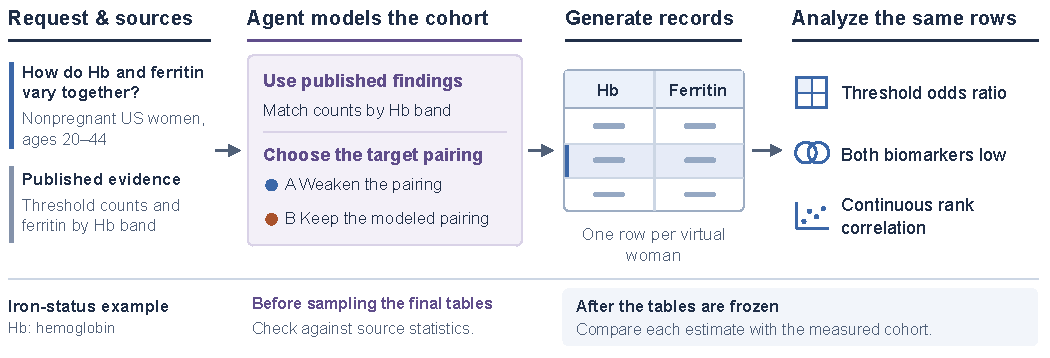
\includegraphics[width=\linewidth]{figures/fig1-agent-method.drawio.pdf}

\caption{The iron-status request through the system. Study findings constrain the model that the agent builds. The agent also chooses how to pair measurements and how to apply the source evidence in the requested population. Each virtual row pairs hemoglobin with ferritin, so the three analyses use the same records. In the sealed iron evaluation the measured target biomarkers became available only after generation.}

\label{fig:2}

\end{figure}

The common method is to build and record a sampling rule suited to the requested analysis. Its statistical form changes with the evidence. For CHNS glycemia, one constructor connected two separately adjusted source regressions by supplying a residual dependence assumption (Supplement S11). For HRS, fitted model exports supplied a starting point for generating repeated visits per person. Each construction delivers its own specification, numerical uses of evidence and executable program. A second author can produce a different joint law from the same packet.


\subsection{Use trial feedback to make a scientific decision}

The coordinator binds the candidate program to a particular version. A numerical worker samples it and reports the diagnostics the protocol allows. In a source replay the worker draws records under the source population rules and calculates the quantity reported in the source study, using its definition and units. A summary of a trial in the target context answers a different question about what that generator produced. A numerical comparison with the paper requires a compatible definition, weighting scheme and source population.


The iron task allowed one source-only review per author. For A, a trial of 100,000 source rows gave a crude odds ratio of 6.58, compared with 6.65 from the published counts. The simulated band-specific geometric means also tracked the reported values. A separate inspection of the sampling rule found that the original upper ferritin tail had infinite variance. A finite trial can look plausible even when very rare draws make the model variance diverge. For concentrations above the cutoff, A used a rescaled square root of the original random draw on the log scale to slow the growth of the upper tail. The replacement preserves the mean log excess, threshold membership and rank order for fixed latent draws, and gives finite variance. This change repaired the mathematical behavior of the generator. The three registered analyses depend on thresholds or ranks, so the repair preserves their results for the same draws.


B's source trial produced an odds ratio of 6.73, with the three band means close to their source values. B retained the initial program. When a source statistic cannot be reproduced under its stated definition, the system records an unavailable check. In Q5 all 132 proposed source comparisons were unavailable because weighting, statistical definitions or details required for implementation were missing or unsupported. For example, the weight convention for a source summary of mean BMI in men was unspecified. The mean in an equally weighted synthetic sample could not stand in for that source estimator. The six Q5 authors could inspect their generated summaries and all retained their programs.


\subsection{Freeze the tables and evaluate a scientific use}

Once a final model has been selected, the coordinator records the program identity and draws all prespecified deliveries. In the iron study each model supplied 5,000 rows at each of three seeds. The program and table hashes were sealed before the measured target biomarkers were accessed. The evaluator ran the three prespecified analyses on the same two columns in every synthetic delivery. It computed the survey quantities using the eligibility, phlebotomy weight, strata and primary sampling units of the measured data. For Q5, the evaluator instead read previously computed reference estimates after the batch was closed. Supplement S12 documents the study-specific implementation paths.


An analysis can be rerun from a delivered table without asking the agent to refit the model to that result. We distinguish successful execution, agreement of a specified point estimate or association pattern, and adequacy for a scientific decision. Our evaluations report the first two, including discrepancies; they do not set a general acceptance threshold for the third. For a threshold analysis the evaluator classifies each generated and measured pair using the same cutoffs. For continuous dependence it uses the original paired concentrations and their ranks. Agreement on threshold counts leaves room for differences in continuous ranks. Table 5 summarizes the demonstrated properties and the uses that remain unvalidated. Marginal and residual variation are reported where available.


The construction, the generated table and the measured participant are different units. Three draws from one frozen model show finite-table sampling variation conditional on that model. Independently authored models show variation across construction decisions; their spread is not a calibrated interval for model uncertainty. Measured participants contribute to the reference estimate under the cohort or survey design, including clustering and repeated observations where applicable. Generating more rows does not add measured participants or reduce uncertainty in the source evidence. These sources of variation answer different questions and are shown separately in the results. Standard errors or tests obtained by treating the synthetic rows as sampled patients do not automatically include uncertainty in source estimates, model selection or population transfer. The present evaluation does not validate confidence-interval coverage, power calculations or clinical decisions from those rows. A data-use statement should identify the synthetic status, source-supported and assumed properties, evaluated analyses, and the uncertainty omitted from any reported interval.


\section{Evaluation design}

Each experiment specifies what the constructor can see and which analyses the delivered table should support (Table 4). We first evaluate complete cohorts built for two glycemia requests, then examine the information contrast and additional biomedical uses. Across studies, a construction is a separately authored model. Repeated draws quantify sampling variation within that model. We report discrepancies in the units of the intended scientific analysis and preserve each study's original decision rule.


\FloatBarrier

\begingroup

\small

\renewcommand{\arraystretch}{1.22}

\begin{xltabular}{\linewidth}{@{}>{\raggedright\arraybackslash}X>{\raggedright\arraybackslash}X>{\raggedright\arraybackslash}X>{\raggedright\arraybackslash}X@{}}

\caption{What the constructor could know, and what the evaluation can establish. Q1–\allowbreak{}Q5 are the identifiers of the frozen experiments. The iron study and the earlier prospective tests have separate protocols. All listed tasks generate complete cohorts.}\label{tab:4} \\

\toprule

\textbf{Study} & \textbf{Construction inputs} & \textbf{Constructions and final deliveries} & \textbf{Analysis} \\

\midrule

\endfirsthead

\multicolumn{4}{l}{\small Table \thetable\ continued}\\

\toprule

\textbf{Study} & \textbf{Construction inputs} & \textbf{Constructions and final deliveries} & \textbf{Analysis} \\

\midrule

\endhead

\bottomrule

\endfoot

Q4: open-retrieval replication & Population/\allowbreak{}measurement definitions and analyses; no bibliographic seeds or target records/\allowbreak{}results & 4 agent; 12 tables of 3,000 & Six glycemia analyses; adjustment patterns \\

Q1: CHNS and ENSANUT & Basic evidence (E0); E0 plus external relations (E1) & 20 agent + 4 prescribed; 72 tables of 3,000 & Six adjusted glycemia coefficients \\

Iron status & External evidence; target eligibility; no target biomarkers & 2 agent; 6 tables of 5,000 & Threshold association, joint burden and continuous ranks \\

Q5: glycemia and lipids & Reviewed external papers, population description, optional retrieval & 6 agent; 18 tables of 3,000 & Six requested effects or correlations \\

Earlier prospective wave & External summaries and population description; exact target results withheld & 5 agent + 1 prescribed per case; 36 tables of 5,000 & HAALSI glucose and Turkana lipid analyses \\

Q3: longitudinal reconstruction & Published HRS fitted-model artifacts & 1 agent + 1 reconstructed; 6 valid tables, 11,509 subjects × 4 visits each & Age–\allowbreak{}HbA1c interactions in memory trajectories \\

Q2: supplied-summary reconstruction & With or without 30 target summaries & 6 agent laws; 18 distinct tables & Reconstruction of supplied summaries \\

\end{xltabular}

\endgroup

CHNS (6,631 adults, ages 35–\allowbreak{}74) uses unweighted estimates for the selected sample. ENSANUT (6,931 adults, ages 25–\allowbreak{}79) assigns equal mass to eight sex-by-age cells. In Q1, each case and information condition has five fresh agent authors and one prescribed statistical law. We average absolute discrepancy over three draws within each law, then across laws within the arm. E0 and E1 authors are not paired. The prescribed law illustrates a statistical completion from the same information; it is not a competitive search over statistical methods.


Supplement S16 gives the eligibility, measurement selection, weighting and uncertainty definition for each reference. In particular, the ENSANUT estimand uses selected adults without a reported prior diabetes diagnosis, with a recorded 8–\allowbreak{}12-hour fast and serum glucose below 126 mg/\allowbreak{}dL, and equal mass in eight age-by-sex cells. It is not a nationally weighted adult-population regression.


The reference conditions differ. Q1–\allowbreak{}Q5 reused project-level references where applicable. For iron status we sealed the protocol and the six deliveries before acquiring the target biomarkers; NHANES was already known to the project. In the earlier prospective wave, a custodian withheld the exact HAALSI and Turkana results, although investigators knew related Turkana findings. We distinguish target sampling intervals, resampling stability bands and model-conditional intervals in the figures. None makes a sample estimate the true population value.


\section{Results}

\subsection{Can generated cohorts support the requested scientific analyses?}

Four fresh authors constructed complete cohorts for the CHNS and ENSANUT requests through open paper retrieval. They received the analyses and population definitions, but no target measurements, coefficients, desired signs or prior models. Their twelve final 3,000-row tables supported all six requested analysis definitions. All 36 seed estimates retained the reference point direction; the effective replication units are four authored laws and two requests, not 36 independent discoveries. A separate implementation reproduced all 366 reported coefficients and diagnostics on the frozen outputs (Supplement S3).


For CHNS, the two construction means for age/\allowbreak{}sex-adjusted BMI were 0.03992 and 0.05338 against a reference of 0.05495 HbA1c percentage points per kg/\allowbreak{}m². The corresponding glucose coefficients were 0.37754 and 0.49241 against 0.40209 percentage points per mmol/\allowbreak{}L. The conditional age coefficients were smaller than the reference: 0.00311 and 0.00563 versus 0.00811 per year. Both authors preserved the three reference point directions, with different magnitude discrepancies across analyses (Figure 3).


For ENSANUT, the BMI coefficient before and after adding glucose adjustment changed from 0.09165 to 0.07509 in E01 and from 0.07140 to 0.04733 in E02, compared with 0.08364 to 0.05664 in the sample reference. Every draw preserved attenuation using the same generated records. This is a multivariable association pattern, not causal mediation or a wholly evidence-independent discovery. Both age coefficients were too large, and residual HbA1c RMS was only approximately 0.295/\allowbreak{}0.324 against 0.488. Direction and adjustment behavior did not ensure adequate individual variability.


\begin{figure}[htbp]

\centering

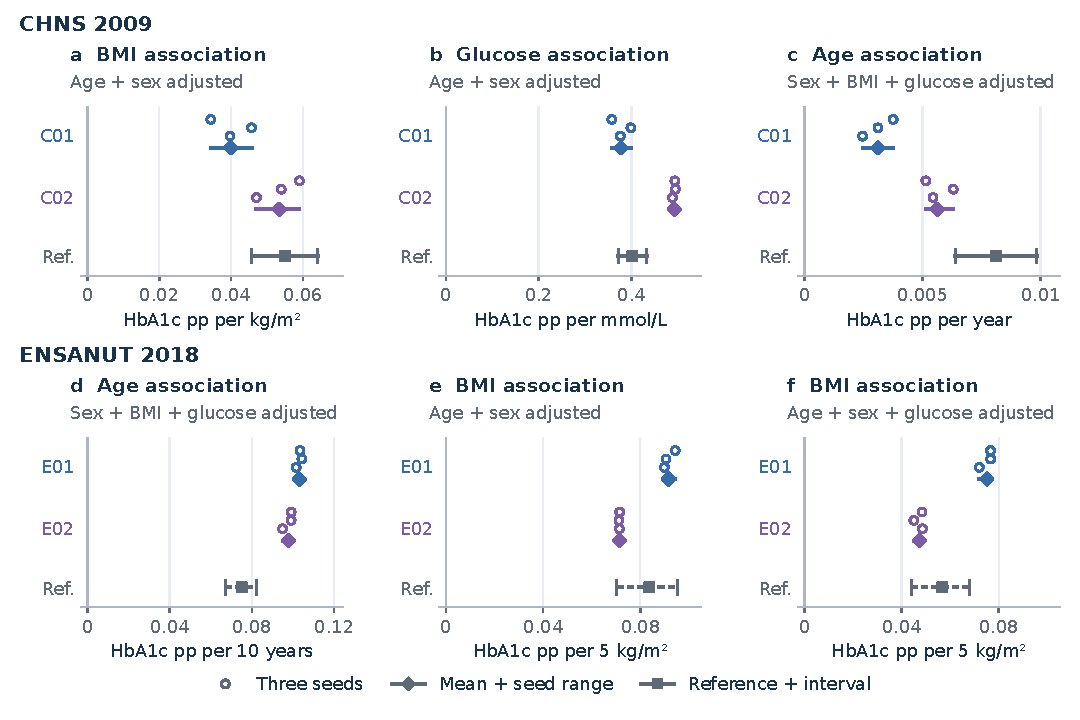
\includegraphics[width=\linewidth]{figures/fig3-analysis-utility.pdf}

\caption{Analysis-specific utility of repeated open-evidence cohort construction. Four Agent authors independently selected external evidence and constructed complete virtual cohorts for CHNS 2009 (C01, C02; a-c) and ENSANUT 2018 (E01, E02; d-f) requests. All six prespecified analyses and all 36 estimates from 12 final tables of 3,000 virtual rows are shown. Open circles are the three fixed seed draws per law (8101-8103, top to bottom); diamonds and colored lines show their means and ranges. Gray squares show the existing sample estimates. Solid reference bars in a-c are community-cluster CR1-t 95\% confidence intervals for the selected, unweighted CHNS analytical sample; dashed bars in d-f are empirical cluster-resampling stability bands from the 399-attempt ENSANUT procedure. These intervals have different interpretations and are not equivalence or acceptance margins. HbA1c effects are in percentage points (pp), with predictor units and adjustment sets shown on each panel. All generated estimates retain the positive reference direction, and both ENSANUT constructions retain BMI-coefficient attenuation after glucose adjustment. Effect magnitudes remain mixed: both CHNS age effects are smaller, and both ENSANUT age effects larger, than their sample references. Seed ranges describe sampling under fixed laws, not uncertainty in evidence or population transfer. The previously exposed references make this developmental replication, not independent clinical validation; all constructions and their additional dispersion and rank-dependence discrepancies remain in the complete evaluation.}

\label{fig:3}

\end{figure}

A separate real-real context analysis evaluated three earlier tables from one evidence-to-generation law, not these four authors. Across 100 community-disjoint CHNS resplits, the median absolute reduced-model BMI difference was 0.007239; symmetric generated-real discrepancy medians were 0.004383–\allowbreak{}0.012727. Age discrepancies were also on a similar numerical scale, while the full-model glucose discrepancy remained appreciably larger than real-real variation. This supplies descriptive context rather than an equivalence threshold, and does not make 100 resplits independent cohorts (Supplement S6).


\subsection{Which regressions improve with additional relationship evidence?}

The next comparison asks whether published associations help constrain the scientific information in a generated cohort beyond basic summaries. Across CHNS and ENSANUT, the sampled agent arms given these additional relationships (E1) had smaller mean absolute discrepancies than the basic-evidence arms (E0) for five of six regression coefficients (Figure 4). For the CHNS glucose slope the error fell from 0.134019 to 0.024079 HbA1c percentage points per mmol/\allowbreak{}L. The CHNS BMI error increased from 0.020380 to 0.031557 percentage points per kg/\allowbreak{}m². All three ENSANUT discrepancies decreased. These are descriptive contrasts between the sampled construction arms; they do not isolate a feedback or revision effect. Some E1 endpoints were closer under the prescribed statistical construction, including CHNS glucose (0.012021 versus 0.024079 for the agent mean) and ENSANUT BMI adjusted for glucose (0.007940 versus 0.025649). Table S1 reports both statistical arms and both agent arms for all six analyses.


Agent arm averages were closer than the delivered statistical specification in six of six E0 comparisons and four of six E1 comparisons. The comparator completes unprovided within-source dependence by independence under its entropy criterion; mixing sources can still induce dependence. Agents can instead choose dependent structures and document their assumptions. In ENSANUT E1, they used the published age slope numerically, whereas the fixed specification left it contextual because source covariates, dispersion and weighting were unbound. These are relevant differences in evidence use under incomplete specification. Five Agent constructions versus one fixed construction per arm do not establish superiority over statistical model search, and every E1 Agent lost to the statistical reference on CHNS glucose and ENSANUT glucose-adjusted BMI.


\begin{figure}[htbp]

\centering

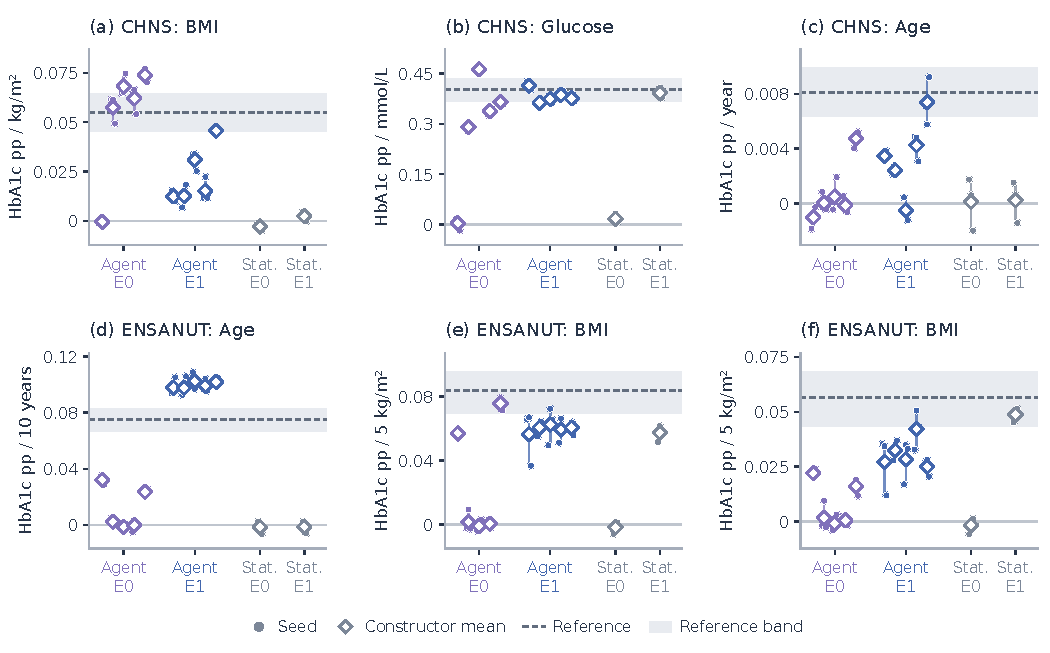
\includegraphics[width=\linewidth]{figures/fig2-evidence-results.pdf}

\caption{Relational evidence and scientific analysis agreement. CHNS panels show BMI adjusted for age/\allowbreak{}sex (a), glucose adjusted for age/\allowbreak{}sex (b), and age adjusted for sex/\allowbreak{}BMI/\allowbreak{}glucose (c). ENSANUT panels show age adjusted for sex/\allowbreak{}BMI/\allowbreak{}glucose (d), BMI adjusted for age/\allowbreak{}sex (e), and BMI additionally adjusted for glucose (f). All six analyses retain native units. E0 contains basic/\allowbreak{}marginal evidence; E1 adds relations. Each agent arm has five independently authored laws and each statistical arm one prescribed law, with all three final draws retained: 24 constructions, 72 tables and 216 coefficient estimates. Dots show seeds, open diamonds constructor means and thin segments seed ranges; dashed lines mark sample references. Reference bands are CHNS community-cluster CR1-t intervals or ENSANUT cluster-resampling stability bands. Author indices do not pair E0 with E1. Table S1 gives every endpoint's mean absolute discrepancy and E1–\allowbreak{}E0 contrast.}

\label{fig:4}

\end{figure}

\subsection{Which analyses can use the same iron-status records?}

Zhu et al. studied 1,671 parous women who used IUDs in northern China, two to four years postpartum [33]. The source counts imply a crude odds ratio of 6.65. The agents' source replays gave 6.58 and 6.73. Both programs used the hemoglobin bands and their ferritin summaries. The Cuban study used inflammation-corrected ferritin [34]. As specified in the shared packet, its odds ratio supplied context for the transfer assumptions (Table 2).


Figure 5 traces the implications of the frozen code. In A, giving low-ferritin observations a relative weight of two thirds preserves the threshold odds ratio, since the factor cancels in the cross-product of counts. It reduces the joint-low proportion from 10.35\% to 7.67\%. For one fifth of rows A then draws hemoglobin independently from the same target hemoglobin distribution. The resulting model implies a joint-low proportion of 6.73\% and an odds ratio of 4.65. B retains the source joint-low proportion of 10.35\% and odds ratio of 6.65. These values follow from the two authored models. The colored markers in panels c to e show estimates from the six previously sealed tables.


The survey reference used the 979 women with both measurements among 1,065 eligible positive-weight women [35]. Missing either measurement excluded 86 women (8.08\% unweighted; 2.47\% of eligible phlebotomy-weight mass). The reported estimates describe this weighted complete-case reference; extending them to all eligible women requires assumptions about the missing measurements (Supplement S9). Comparison on the log-odds-ratio scale was primary. All six delivered odds ratios (A 4.835–\allowbreak{}4.866, B 6.011–\allowbreak{}6.565) fell below the survey's lower confidence limit of 9.28 (estimate 17.79, 95\% CI 9.28–\allowbreak{}34.11). A came closer on the joint-low proportion (6.66–\allowbreak{}6.88\% versus 7.63\%), while B came closer on the continuous Spearman correlation (0.391–\allowbreak{}0.430 versus 0.398). For B the joint-low proportion was 10.02–\allowbreak{}10.44\%, and for A the correlation was 0.156–\allowbreak{}0.195. The sources reported no continuous rank coefficient. Their ferritin summaries by hemoglobin band constrain ranks indirectly, leaving within-band dependence to the author. The same two columns in each delivery supplied all three estimates.


\begin{figure}[htbp]

\centering

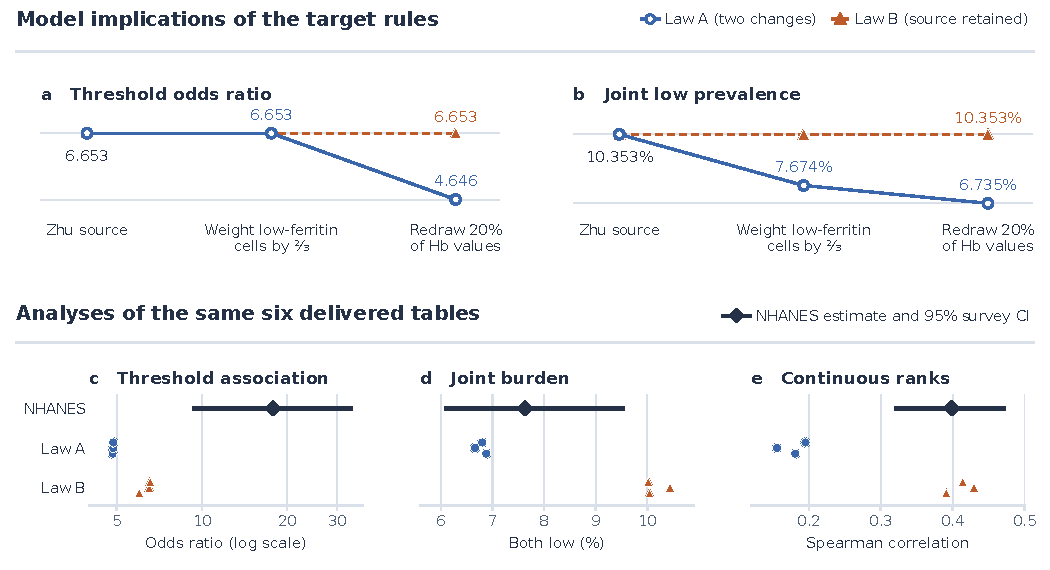
\includegraphics[width=\linewidth]{figures/fig3-iron-utility.pdf}

\caption{How two transfer choices affect analyses on the same iron-status records. Panels a and b are a post hoc calculation from the source counts and frozen rules. Panels c to e show three sealed tables of 5,000 rows per law and the NHANES estimate with its design-based 95\% interval. Low hemoglobin is below 12 g/\allowbreak{}dL and low raw ferritin below 15 µg/\allowbreak{}L. The two secondary analyses had no prespecified equivalence margin.}

\label{fig:5}

\end{figure}

\subsection{Which findings carry across requests and reference conditions?}

For glycemia and lipids, three authors per request generated 18 tables in total. All 54 primary estimates agreed in point direction with the corresponding sample estimates across six distinct analyses (Figure 6). The tables supported age- and sex-adjusted BMI models and further adjustment for glucose. The three constructor-mean correlations of total and HDL cholesterol after adjustment for age, sex and BMI were 0.108–\allowbreak{}0.141, against 0.512 in the measured sample. The total-cholesterol slope's reference interval crossed zero. A post hoc check of the sealed lipid tables found HDL above total cholesterol in 69 of 27,000 synthetic rows (0.256\%). Both concentrations were expressed in mmol/\allowbreak{}L. This check measures the biological consistency of individual pairs separately from the prespecified association results.


A close coefficient did not imply that individual variation was reproduced. H03's mean glucose-adjusted BMI coefficient was 0.05098 versus 0.05664 HbA1c percentage points per 5 kg/\allowbreak{}m² in the reference. Its mean HbA1c SD was 0.3523 versus 0.5274 percentage points, and its full-model residual RMS was 0.3006 versus 0.4885 (Figure S2). These diagnostics qualify its regression-use result: the tables retained less marginal and residual variation. The lower residual variation also limits inferential uses: a close slope does not establish calibrated standard errors, confidence intervals or power. Studies of individual heterogeneity and tails likewise require their own validation.


\begin{figure}[htbp]

\centering

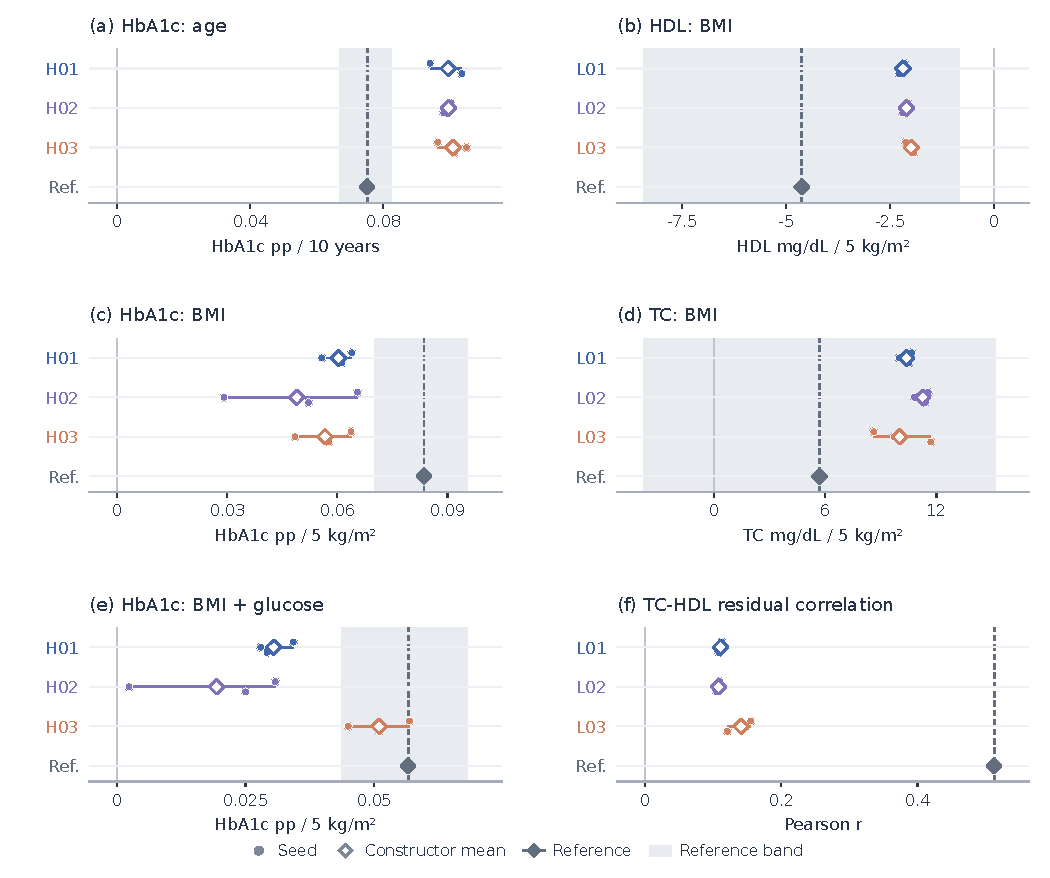
\includegraphics[width=\linewidth]{figures/fig3-cross-task.pdf}

\caption{Analysis-specific behavior across glycemia and lipid requests. HbA1c panels in the left column show age adjusted for sex/\allowbreak{}BMI/\allowbreak{}glucose (a), BMI adjusted for age/\allowbreak{}sex (c), and BMI additionally adjusted for glucose (e). The right column shows age/\allowbreak{}sex-adjusted HDL and TC BMI slopes (b,d) and residual Pearson correlation after age/\allowbreak{}sex/\allowbreak{}BMI adjustment (f). All six laws and 54 estimates from 18 tables are retained. Circles show seeds, open diamonds means and thin segments seed ranges; dark diamonds and dashed lines mark sample references. HbA1c units are percentage points per 10 years or 5 kg/\allowbreak{}m²; lipid slopes are mg/\allowbreak{}dL per 5 kg/\allowbreak{}m². Bands are ENSANUT empirical cluster-resampling stability bands and lipid HC3 assumption-conditional sensitivity intervals. The TC band crosses zero; no residual-correlation interval is available. Seed ranges describe sampling under each frozen law. Table S5 supplies all numerical summaries and Figure S2 the dispersion results.}

\label{fig:6}

\end{figure}

The earlier prospective wave tested a stricter question. In HAALSI adults aged 40 or older [30,31], all 15 agent draws recovered the positive directions of the adjusted BMI and age associations with capillary glucose; only eight recovered the negative difference between female and male BMI slopes. The rule required four of five laws per case to meet all prespecified margins on every seed. Three passed in HAALSI and none in Turkana [32], so the planned expansion stopped. Even a zero-effect rule met the HAALSI margin for all three endpoints. The earlier method and its gate remain a separate prospective result, not a fresh evaluation of the later workflow on the same Turkana participants.


\subsection{What changes when the scientific relationship is already supplied?}

In the HRS longitudinal benchmark both methods received the published model exports [1]. Below the 6.5\% HbA1c knot, the age–\allowbreak{}HbA1c interaction in memory trajectories averaged −0.04464 for agent tables and −0.04050 for the reconstructed published generator, against the supplied −0.04684. Above the knot the mean signs differed; five of six intervals included zero (Figure S5). This is a matched reconstruction check, not transfer from partial evidence. Similarly, supplying 30 target summaries in Q2 allowed joint reconstruction of the five highlighted regression and correlation analyses (Table S2). In Q4, open retrieval yielded twelve distinct original studies across four authors and twelve complete tables (Tables S3–\allowbreak{}S4); the design did not isolate the effect of retrieval. HRS and Q2 test reconstruction when target-model information is supplied; Q4 instead demonstrates a way to obtain external evidence without supplying more information about the target.


\FloatBarrier

\begingroup

\small

\renewcommand{\arraystretch}{1.22}

\begin{xltabular}{\linewidth}{@{}>{\raggedright\arraybackslash}X>{\raggedright\arraybackslash}X>{\raggedright\arraybackslash}X@{}}

\caption{Observed scientific properties and unvalidated uses. These descriptive conclusions add no pass/\allowbreak{}fail criteria. Agreement concerns the stated sample reference or supplied model, not known population truth.}\label{tab:5} \\

\toprule

\textbf{Experiment and intended analysis} & \textbf{Observed property} & \textbf{Use not established by this result} \\

\midrule

\endfirsthead

\multicolumn{3}{l}{\small Table \thetable\ continued}\\

\toprule

\textbf{Experiment and intended analysis} & \textbf{Observed property} & \textbf{Use not established by this result} \\

\midrule

\endhead

\bottomrule

\endfoot

Q4: six glycemia regressions under open retrieval & Four authored laws produced complete tables retaining all six reference point directions. Both ENSANUT laws retained BMI-coefficient attenuation after glucose adjustment; effect magnitudes, ranks and dispersion remained mixed. & Reliable effect-size estimation for an unseen population, causal mediation, or calibrated uncertainty. The two requests used previously exposed references. \\

Q1: comparison with additional relationship evidence & The sampled E1 agent arms had smaller mean absolute discrepancy than E0 on five of six coefficients; CHNS BMI discrepancy increased. Comparisons with the fixed statistical completion varied by endpoint. & A general probability of improvement, universal method superiority, or a feedback/\allowbreak{}revision effect. Authors were unpaired, and six endpoints do not constitute six independent clinical studies. \\

Iron: threshold association, joint burden and continuous ranks from the same paired columns & A was closer on joint-low prevalence; B was closer on Spearman correlation. Both substantially understated the primary odds ratio; all six delivered ORs lay below the reference interval's lower limit. & Adequacy of one law for all three analyses, direct source-to-target transport, or a prospective rule for choosing the better construction without target measurements. No equivalence margin was specified. \\

Q5: glycemia and lipid regressions and residual dependence & All focal point directions agreed. H03's glucose-adjusted BMI coefficient was relatively close despite reduced HbA1c dispersion; lipid residual correlations remained 0.108–\allowbreak{}0.141 versus 0.512 in the sample reference. & Adequate joint variation, individual heterogeneity or tails, or reliable magnitude recovery inferred from direction alone. The TC reference interval included zero. \\

HRS/\allowbreak{}Q3 and Q2: analyses whose model information or summaries were supplied & HRS tables retained the below-knot interaction's negative direction, with unstable upper-branch behavior. Q2 reconstructed the five highlighted supplied regression/\allowbreak{}correlation summaries jointly. & Recovery of an unconstrained hidden relationship or independent population validation. The relevant target-model information was legitimate construction input. \\

\end{xltabular}

\endgroup

\section{Discussion}

The central result is repeated conversion of incomplete scientific information into executable cohorts with partial agreement on specified analyses. In the open-retrieval cases, different authored models preserved several effect magnitudes and the reduction in the BMI coefficient after glucose adjustment. In the separate information experiment, arms given relationship evidence had smaller discrepancies on five of six analyses. These findings locate practical value in the evidence-to-model construction: the user can specify the research problem without first writing a complete joint generator. The host-reviewed workflow and its outcomes do not yet establish how reliably a new user can obtain an accurate scientific inference without a target comparison.


The favorable fixed-comparator results occur under incomplete joint specification. They motivate examining how an Agent uses evidence and supplies dependence assumptions, not assuming that language-model generation replaces statistical modeling. The Agent-generated cohorts themselves are statistical models sampled by numerical tools. The implementation contribution is assigning the scientific construction to an author that can interpret different studies and requests, while preserving an executable result. Fully supplied summaries and fitted models are useful reconstruction controls; conventional calibration also performs well in those settings.


Whole-cohort generation and variable extension share this evidence-to-model problem. A richer historical pilot also showed that literal synthetic training rows can retain predictive information on later real participants, but its outcome-conditioned training summaries differ from our literature-driven inputs (Supplement S14). These modes show a practical range of uses without establishing that one unchanged controller or one model law works everywhere. Recent adaptive and source-context prototypes demonstrate additional executed capabilities separately (Supplement S15).


Some scientific properties remain poorly determined. The iron model closer on joint prevalence was not the model closer on continuous ranks; both missed the primary target odds ratio. Lipid residual dependence and glycemia dispersion also remained inaccurate. The diagnoses point to evidence adequacy and joint/\allowbreak{}transfer assumptions as leading explanations, without uniquely identifying their contributions. A controlled diagnostic with exact compatible summaries found that ordinary constructors already reconciled separate projections into the same joint law; adding a consistency instruction gave no improvement (Supplement S13). These results support a simple workflow with explicit assumptions and use-specific evaluation. They do not show that a source-consistency label can predict reliability before a target comparison.


\section{Limitations and Ethical Considerations}

The evidence cannot identify every joint relationship. Sources differ in eligibility, age, geography, specimen handling and adjustment; reference samples have sampling uncertainty. The iron reference also conditions on both biomarkers being observed. Its small weighted missing fraction does not establish absence of selection bias, and no additional item-nonresponse sensitivity analysis was performed. A small number of agent constructions share a model service, and repeated draws do not represent independent clinical cohorts. The protocols and controllers differ across studies; the main evidence and open-retrieval results are developmental evaluations on previously exposed project references. Their shared procedure should not be mistaken for a multi-case confirmation of the newest adaptive controller. Author-model metadata are incomplete in central experiments: the Q1 dispatches record an inherited host model without its exact backend identity, and Q4 records fresh author contexts without a complete model/\allowbreak{}inference configuration. Supplement S17 separates program replay from reproduction of original authoring sessions and identifies the recorded budgets and review stages. No held-out trial shows that review improves outcomes or that the workflow saves a measured amount of human time. For research planning, the source-based and assumed parts should travel with the records. Values must be labeled synthetic and must not be presented as measured individual biomarkers, clinical diagnoses or substitutes for independent patient evidence. Original cohort access and reuse conditions continue to apply; the public artifacts contain code and aggregate results rather than participant-level tables.


\section{Generative AI Usage}

Language models participated in research planning and manuscript editing and were an object of the experiments. In the scientific workflow, agent authors interpreted evidence, selected or received studies according to protocol, proposed statistical models, and wrote or revised generator code. For program-based studies, deterministic tools sampled the records; the historical direct-row study used literal Agent-authored values. Deterministic tools computed the reported analyses, and separate implementations checked the numerical results where specified. Study protocols and source records document these roles. The final author list, study-specific declarations, and applicable oversight and data-use statements must be confirmed before submission.


\section*{Supporting materials and reproducibility}

The \href{https://github.com/ziwang11112/evidence-guided-virtual-cohorts-2026}{public research repository} contains protocols, executable code and aggregate audits. The iron \href{https://github.com/ziwang11112/evidence-guided-virtual-cohorts-2026/commit/bedd845768c1c938768f58fce685f53cbf97f3df}{protocol seal} and \href{https://github.com/ziwang11112/evidence-guided-virtual-cohorts-2026/commit/c88192edeb0bc63b60d0bfe6e3a7282ced9d2975}{delivery seal} precede target evaluation. Supplements retain all prespecified outcomes, unfavorable cases and implementation incidents. This manuscript revision clarifies analysis-use claims, operational roles, reference definitions and reproducibility using existing frozen results. No new clinical cohort was generated or target refitted. Supplement S13 reports a separate artificial mechanism diagnostic; Supplements S14–\allowbreak{}S15 distinguish the historical predictive-use study and later implementation development.


\clearpage

\section*{References}

\begingroup

\begin{enumerate}[label=\arabic*.,leftmargin=2.1em,itemsep=.2em,parsep=0pt]

\item Filshtein TJ, Li X, Zimmerman SC, Ackley SF, Glymour MM, Power MC. Proof of concept example for use of simulation to allow data pooling despite privacy restrictions. \emph{Epidemiology}. 2021;32(5):638–\allowbreak{}647. \href{https://pmc.ncbi.nlm.nih.gov/articles/PMC8338788/}{DOI and full text}.

\item Zhao Z et al. SynthIPD: training-free synthetic individual patient data generation. arXiv:2509.16466v2, 24 July 2026. \href{https://arxiv.org/html/2509.16466v2}{Versioned full text}. Publication beyond this preprint was not established in the positioning audit.

\item Phillippo DM et al. Multilevel network meta-regression for population-adjusted treatment comparisons. \emph{Journal of the Royal Statistical Society: Series A}. 2020;183(3):1189–\allowbreak{}1210. \href{https://rss.onlinelibrary.wiley.com/doi/full/10.1111/rssa.12579}{DOI/\allowbreak{}full text}.

\item Holt S, Ruiz Luyten M, Berthon A, van der Schaar M. G-Sim: Generative Simulations with Large Language Models and Gradient-Free Calibration. \emph{Proceedings of ICML}. PMLR 267;2025:23513–\allowbreak{}23561. \href{https://proceedings.mlr.press/v267/holt25b.html}{Published record}.

\item Tang Y, Kong M, He J, Nie T, Ma W, Sun L. LLMSynthor: Macro-Aligned Micro-Records Synthesis with Large Language Models. KDD 2026. \href{https://doi.org/10.1145/3770855.3818965}{DOI}; \href{https://arxiv.org/html/2505.14752v4}{full text v4}.

\item Callender T, Boyd A, Davis R, Ruhrberg Estevez S, Lavista Ferres JM, van der Schaar M. SynthCraft: An AI partner for synthetic data generation to support data access and augmentation in healthcare. \emph{PLOS Digital Health}. 2026;5(3):e0001290. \href{https://journals.plos.org/digitalhealth/article?id=10.1371/journal.pdig.0001290}{Published article}.

\item Bao Y, Ma X, Li H, Zhou M, Hu C, Wu H, Tang J, Hou X, Xiang K, Jia W. Glycated haemoglobin A1c for diagnosing diabetes in Chinese population: cross sectional epidemiological survey. \emph{BMJ}. 2010;340:c2249. \href{https://doi.org/10.1136/bmj.c2249}{DOI}; \href{https://pubmed.ncbi.nlm.nih.gov/20478961/}{bibliographic record}.

\item Wang P, Li Y, Wang M, Song L, Dong Y, Han X, Tuomilehto J, Wang Y, Du Y, Qiu C. Comparing glycemic traits in defining diabetes among rural Chinese older adults. \emph{PLOS ONE}. 2024;19(1):e0296694. \href{https://journals.plos.org/plosone/article?id=10.1371/journal.pone.0296694}{Published article}.

\item Jansen H, Stolk RP, Nolte IM, Kema IP, Wolffenbuttel BHR, Snieder H. Determinants of HbA1c in nondiabetic Dutch adults: genetic loci and clinical and lifestyle parameters, and their interactions in the lifelines cohort study. \emph{Journal of Internal Medicine}. 2013;273(3):283–\allowbreak{}293. \href{https://onlinelibrary.wiley.com/doi/10.1111/joim.12010}{Published article}.

\item Pani LN, Korenda L, Meigs JB, Driver C, Chamany S, Fox CS, Sullivan L, D'Agostino RB, Nathan DM. Effect of aging on A1C levels in individuals without diabetes: evidence from the Framingham Offspring Study and the National Health and Nutrition Examination Survey 2001-2004. \emph{Diabetes Care}. 2008;31(10):1991–\allowbreak{}1996. \href{https://doi.org/10.2337/dc08-0577}{DOI}; \href{https://pubmed.ncbi.nlm.nih.gov/18628569/}{bibliographic record}.

\item NGSP. The IFCC and NGSP, Table 2. \href{https://ngsp.org/ifccngsp.asp}{Official measurement-scale guidance}.

\item Li T, Quan H, Zhang H, Lin L, Lin L, Ou Q, Chen K. Type 2 diabetes is more predictable in women than men by multiple anthropometric and biochemical measures. \emph{Scientific Reports}. 2021;11:6062. \href{https://doi.org/10.1038/s41598-021-85581-z}{DOI}; \href{https://pmc.ncbi.nlm.nih.gov/articles/PMC7960723/}{original full text}.

\item Sakane N, Sato J, Tsushita K, Tsujii S, Kotani K, Tominaga M, Kawazu S, Sato Y, Usui T, Kamae I, Yoshida T, Kiyohara Y, Sato S, Tsuzaki K, Nirengi S, Takahashi K, Kuzuya H, JDPP Research Group. Determinants of Glycated Hemoglobin in Subjects With Impaired Glucose Tolerance: Subanalysis of the Japan Diabetes Prevention Program. \emph{Journal of Clinical Medicine Research}. 2017;9(4):360–\allowbreak{}365. \href{https://doi.org/10.14740/jocmr2928w}{DOI}; \href{https://pmc.ncbi.nlm.nih.gov/articles/PMC5330780/}{original full text}.

\item Wisgerhof W, Ruijgrok C, den Braver NR, Borgonjen—van den Berg KJ, van der Heijden AAWA, Elders PJM, Beulens JWJ, Alssema M. Phenotypic and lifestyle determinants of HbA1c in the general population–\allowbreak{}The Hoorn Study. \emph{PLOS ONE}. 2020;15(6):e0233769. \href{https://doi.org/10.1371/journal.pone.0233769}{DOI}; \href{https://pmc.ncbi.nlm.nih.gov/articles/PMC7272077/}{original full text}.

\item Yang S, Zhang Z, Prenkaj B, Kasneci G. Doubling Your Data in Minutes: Ultra-fast Tabular Data Generation via LLM-Induced Dependency Graphs. \emph{Proceedings of the 2025 Conference on Empirical Methods in Natural Language Processing}. 2025:10337–\allowbreak{}10358. \href{https://aclanthology.org/2025.emnlp-main.525/}{Official article and PDF}; \href{https://doi.org/10.18653/v1/2025.emnlp-main.525}{DOI}.

\item Wu et al. Effect of age on the diagnostic efficiency of HbA1c for diabetes in a Chinese middle-aged and elderly population: The Shanghai Changfeng Study. \emph{PLoS ONE}. 2017. \href{https://pmc.ncbi.nlm.nih.gov/articles/PMC5591004/}{Admitted original}.

\item Skogberg et al. The association between anthropometric measures and glycated haemoglobin (HbA1c) is different in Russian, Somali and Kurdish origin migrants compared with the general population in Finland: a cross-sectional population-based study. \emph{BMC Public Health}. 2019. \href{https://pmc.ncbi.nlm.nih.gov/articles/PMC6458679/}{Admitted original}.

\item Zhang et al. The Association of Retinopathy and Plasma Glucose and HbA1c: A Validation of Diabetes Diagnostic Criteria in a Chinese Population. \emph{Journal of Diabetes Research}. 2016. \href{https://pmc.ncbi.nlm.nih.gov/articles/PMC5078665/}{Admitted original}.

\item Venkataraman et al. Ethnicity modifies the relation between fasting plasma glucose and HbA1c in Indians, Malays and Chinese. \emph{Diabetic Medicine}. 2012. \href{https://pmc.ncbi.nlm.nih.gov/articles/PMC3504343/}{Admitted original}.

\item Liu et al. Ideal glycated hemoglobin cut-off points for screening diabetes and prediabetes in a Chinese population. \emph{Journal of Diabetes Investigation}. 2016. \href{https://pmc.ncbi.nlm.nih.gov/articles/PMC5009131/}{Admitted original}.

\item Huang et al. Hemoglobin A1c Levels Associated with Age and Gender in Taiwanese Adults without Prior Diagnosis with Diabetes. \emph{International Journal of Environmental Research and Public Health}. 2021. \href{https://pmc.ncbi.nlm.nih.gov/articles/PMC8038122/}{Admitted original}.

\item Ghazanfari et al. A Comparison of HbA1c and Fasting Blood Sugar Tests in General Population. \emph{International Journal of Preventive Medicine}. 2010. \href{https://pmc.ncbi.nlm.nih.gov/articles/PMC3075530/}{Admitted original}.

\item Masuch et al. Preventing misdiagnosis of diabetes in the elderly: age-dependent HbA1c reference intervals derived from two population-based study cohorts. \emph{BMC Endocrine Disorders}. 2019. \href{https://pmc.ncbi.nlm.nih.gov/articles/PMC6371438/}{Admitted original}.

\item Marini et al. Association between hemoglobin glycation index with insulin resistance and carotid atherosclerosis in non-diabetic individuals. \emph{PLoS ONE}. 2017. \href{https://pmc.ncbi.nlm.nih.gov/articles/PMC5398507/}{Admitted original}.

\item Greiner et al. Associations between low HDL, sex and cardiovascular risk markers are substantially different in sub-Saharan Africa and the UK: analysis of four population studies. \emph{BMJ Global Health}. 2021;6:e005222. \href{https://doi.org/10.1136/bmjgh-2021-005222}{DOI}; \href{https://gh.bmj.com/content/6/6/e005222corr1}{published correction to author names}.

\item Obirikorang et al. Obesity and Cardio-Metabolic Risk Factors in an Urban and Rural Population in the Ashanti Region-Ghana: A Comparative Cross-Sectional Study. \emph{PLOS ONE}. 2015;10:e0129494. \href{https://doi.org/10.1371/journal.pone.0129494}{DOI}; \href{https://journals.plos.org/plosone/article?id=10.1371/journal.pone.0129494}{admitted original}.

\item Agongo et al. The burden of dyslipidaemia and factors associated with lipid levels among adults in rural northern Ghana: An AWI-Gen sub-study. \emph{PLOS ONE}. 2018;13:e0206326. \href{https://doi.org/10.1371/journal.pone.0206326}{DOI}; \href{https://journals.plos.org/plosone/article?id=10.1371/journal.pone.0206326}{admitted original}.

\item Agongo et al. Correction: The burden of dyslipidaemia and factors associated with lipid levels among adults in rural northern Ghana: An AWI-Gen sub-study. \emph{PLOS ONE}. 2019;14:e0213233. \href{https://doi.org/10.1371/journal.pone.0213233}{DOI}; \href{https://pmc.ncbi.nlm.nih.gov/articles/PMC6392312/}{correction}. The correction concerns hip/\allowbreak{}waist entries and a citation; those entries were not used in the lipid constructions.

\item Gu T, Taylor JMG, Mukherjee B. A synthetic data integration framework to leverage external summary-level information from heterogeneous populations. \emph{Biometrics}. 2023;79:3831–\allowbreak{}3845. \href{https://doi.org/10.1111/biom.13852}{DOI}.

\item Gómez-Olivé FX et al. Cohort Profile: Health and Ageing in Africa: A Longitudinal Study of an INDEPTH Community in South Africa (HAALSI). \emph{International Journal of Epidemiology}. 2018;47:689–\allowbreak{}690j. \href{https://doi.org/10.1093/ije/dyx247}{Cohort profile}.

\item Harvard Center for Population and Development Studies. HAALSI Baseline Survey. Harvard Dataverse, 2016, version 3.0. \href{https://doi.org/10.7910/DVN/F5YHML}{Dataset}.

\item Lea AJ, Martins D, Kamau J, Gurven M, Ayroles JF. Urbanization and market integration have strong, nonlinear effects on cardiometabolic health in the Turkana. \emph{Science Advances}. 2020;6:eabb1430. \href{https://doi.org/10.1126/sciadv.abb1430}{Article}. \href{https://doi.org/10.5061/dryad.2z34tmpjk}{Dataset}.

\item Zhu JH et al. Iron, folate, and B12 deficiencies and their associations with anemia among women of childbearing age in a rural area in northern China. International Journal for Vitamin and Nutrition Research. 2010;80:144–\allowbreak{}154. \href{https://doi.org/10.1024/0300-9831/a000014}{Article}.

\item Pita-Rodríguez GM et al. Prevalence of Anemia and Iron Deficiency in Women of Reproductive Age in Cuba and Associated Factors. International Journal of Environmental Research and Public Health. 2023;20:5110. \href{https://doi.org/10.3390/ijerph20065110}{Article}.

\item National Center for Health Statistics. NHANES, August 2021–\allowbreak{}August 2023: Ferritin (FERTIN\_L); Complete Blood Count (CBC\_L); Demographic Variables and Sample Weights (DEMO\_L). \href{https://wwwn.cdc.gov/Nchs/Data/Nhanes/Public/2021/DataFiles/FERTIN\_L.htm}{Ferritin and phlebotomy weights}; \href{https://wwwn.cdc.gov/Nchs/Data/Nhanes/Public/2021/DataFiles/CBC\_L.htm}{complete blood count}; \href{https://wwwn.cdc.gov/Nchs/Data/Nhanes/Public/2021/DataFiles/DEMO\_L.htm}{demographics}.

\item Jiang J, Gao C, Rasmussen E, Xie SZ, Sun J. KMGen: A Skill-based Approach for Synthetic Individual Patient Data Generation. \emph{Proceedings of the 11th Machine Learning for Healthcare Conference}. PMLR 340;2026:755–\allowbreak{}814. \href{https://proceedings.mlr.press/v340/jiang26a.html}{Official proceedings}.

\item Jones M, Dawson R, Mills J. A large language model framework for sample-free population synthesis. \emph{PLOS ONE}. 2026;21(6):e0341704. \href{https://journals.plos.org/plosone/article?id=10.1371/journal.pone.0341704}{Published article}.

\item Jones M, Dawson R, Mills J. Correction: A large language model framework for sample-free population synthesis. \emph{PLOS ONE}. 2026;21(8):e0356492. \href{https://journals.plos.org/plosone/article?id=10.1371/journal.pone.0356492}{Published correction}.

\end{enumerate}

\endgroup

\clearpage

\appendix

\section*{Supplementary results}

\setcounter{figure}{0}

\renewcommand{\thefigure}{S\arabic{figure}}

\setcounter{table}{0}

\renewcommand{\thetable}{S\arabic{table}}

The supplement retains the complete numerical comparisons and supporting displays under their original study identities. Figure and table numbers follow their new placement; no construction, primary result or unavailable comparison is removed by the shorter main narrative. Q1–\allowbreak{}Q5 remain distinct experiments with their original information conditions.


\subsection*{S1. Complete external-evidence contrast}

All 24 Q1 constructions produced their three scheduled final tables. The 72 final tables were distinct and supported every requested regression and diagnostic; seven exploratory tables brought physical executions to 79. Additional relational evidence reduced constructor-averaged mean absolute discrepancy for five of the six designated coefficients (Table S1). CHNS glucose discrepancy decreased from 0.134019 to 0.024079 HbA1c percentage points per mmol/\allowbreak{}L. All three ENSANUT contrasts improved. CHNS BMI discrepancy increased from 0.020380 to 0.031557.


\FloatBarrier

\begingroup

\small

\renewcommand{\arraystretch}{1.22}

\begin{xltabular}{\linewidth}{@{}>{\hsize=1.350000\hsize\linewidth=\hsize\raggedright\arraybackslash}X>{\hsize=0.941667\hsize\linewidth=\hsize\raggedright\arraybackslash}X>{\hsize=0.941667\hsize\linewidth=\hsize\raggedright\arraybackslash}X>{\hsize=0.941667\hsize\linewidth=\hsize\raggedright\arraybackslash}X>{\hsize=0.941667\hsize\linewidth=\hsize\raggedright\arraybackslash}X>{\hsize=0.941667\hsize\linewidth=\hsize\raggedright\arraybackslash}X>{\hsize=0.941667\hsize\linewidth=\hsize\raggedright\arraybackslash}X@{}}

\caption{Complete main-study information and statistical comparisons. All numerical columns report mean absolute discrepancy in HbA1c percentage points per stated predictor increment, except the agent E1−E0 difference between those discrepancies. For each agent arm, absolute discrepancies are averaged over three draws within each of five constructions and then across constructions. Each statistical arm contains one prescribed construction and three draws. E1−E0 is calculated before rounding; E0 and E1 authors are not paired. The contrasts are descriptive. Rows retain their native units and are not pooled.}\label{tab:6} \\

\toprule

\textbf{Case / focal analysis} & \textbf{Predictor increment} & \textbf{Agent E0} & \textbf{Agent E1} & \textbf{Agent E1 − E0} & \textbf{Statistical E0} & \textbf{Statistical E1} \\

\midrule

\endfirsthead

\multicolumn{7}{l}{\small Table \thetable\ continued}\\

\toprule

\textbf{Case / focal analysis} & \textbf{Predictor increment} & \textbf{Agent E0} & \textbf{Agent E1} & \textbf{Agent E1 − E0} & \textbf{Statistical E0} & \textbf{Statistical E1} \\

\midrule

\endhead

\bottomrule

\endfoot

CHNS BMI, adjusted age/\allowbreak{}sex & 1 kg/\allowbreak{}m² & 0.020380 & 0.031557 & +0.011178 & 0.057877 & 0.052555 \\

CHNS glucose, adjusted age/\allowbreak{}sex & 1 mmol/\allowbreak{}L & 0.134019 & 0.024079 & −0.109939 & 0.384750 & 0.012021 \\

CHNS age, adjusted sex/\allowbreak{}BMI/\allowbreak{}glucose & 1 year & 0.007281 & 0.004854 & −0.002426 & 0.007986 & 0.007878 \\

ENSANUT age, adjusted sex/\allowbreak{}BMI/\allowbreak{}glucose & 10 years & 0.063944 & 0.024670 & −0.039274 & 0.076797 & 0.076680 \\

ENSANUT BMI, adjusted age/\allowbreak{}sex & 5 kg/\allowbreak{}m² & 0.056883 & 0.023732 & −0.033151 & 0.085378 & 0.026202 \\

ENSANUT BMI, adjusted age/\allowbreak{}sex/\allowbreak{}glucose & 5 kg/\allowbreak{}m² & 0.048797 & 0.025649 & −0.023147 & 0.058345 & 0.007940 \\

\end{xltabular}

\endgroup

The effect displays explain what these changes mean. CHNS E1 glucose constructor means were 0.363363–\allowbreak{}0.414189 around the 0.402093 reference. Its BMI means were positive but lower, 0.012400–\allowbreak{}0.045757 versus 0.054946. Conditional-age means ranged from −0.000509 to 0.007393 versus 0.008107; one author retained a negative mean and two negative seeds. All ENSANUT E1 focal coefficients were positive, although its age means of 0.097769–\allowbreak{}0.102452 per decade exceeded 0.075132 and its BMI means remained below their references. Preserving a direction and recovering its magnitude are distinct aspects of usefulness.


Every E1 author used at least one relationship as a numerical constraint. The complete uptake records include constraints, unfitted analytic checks and contextual uses, including the case-specific projection calculation in Supplement S11. Statistical references also achieved useful results: under E1, the prescribed constructions had lower seed-averaged discrepancies than every corresponding agent for CHNS glucose and ENSANUT conditional BMI. Other comparisons favored agent constructions. The observed contrasts support the reported analysis-specific agreements and a descriptive association between added relationship information and smaller errors in these sampled arms.


\subsection*{S2. Complete supplied-summary reconstruction}

\begin{figure}[htbp]

\centering

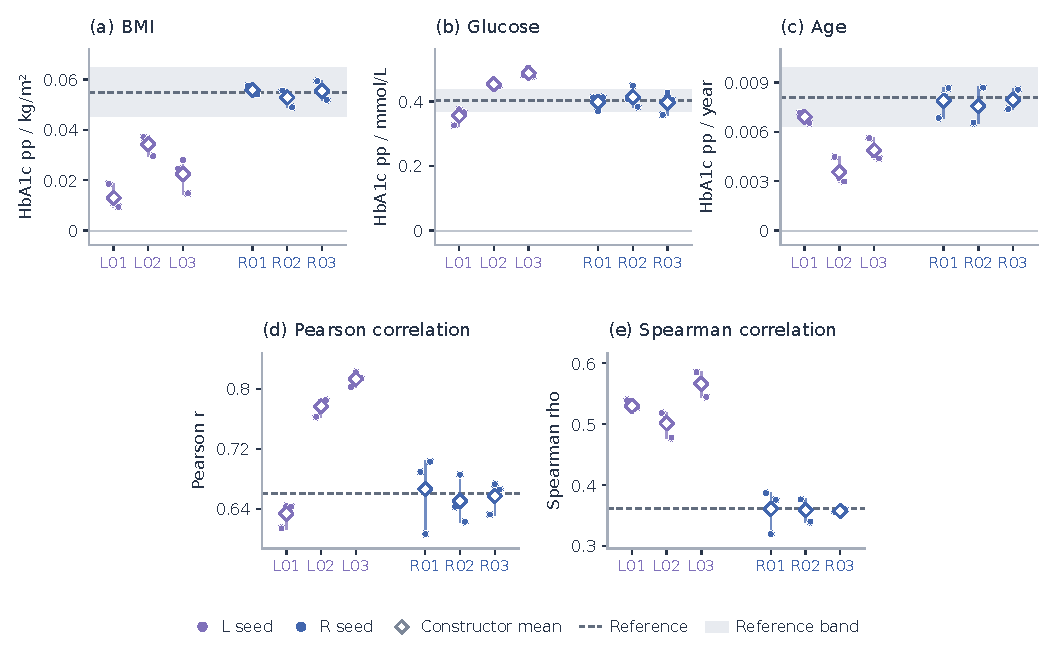
\includegraphics[width=\linewidth]{figures/fig4-summary-results.pdf}

\caption{Supplied summaries become jointly analyzable data. Five panels show BMI, glucose and age regression coefficients plus glucose–\allowbreak{}HbA1c Pearson and Spearman correlations. L01–\allowbreak{}L03 use literature; R01–\allowbreak{}R03 additionally receive 30 target summaries and metadata. Points show all three final draws, diamonds constructor means and segments seed ranges. Dashed lines mark reference summaries available to R; regression bands are CHNS community-cluster CR1-t intervals, with no supplied correlation interval. All six constructors, 18 distinct delivery tables, 30 means and 90 seed statistics appear once. Initial and final deliveries were identical after retention; Table S2 gives the complete five-analysis numerical comparison.}

\label{fig:7}

\end{figure}

The separate CHNS experiment gave three authors external literature (L) and three authors that literature plus 30 target summaries and their metadata (R). Each author delivered three tables and had one additional diagnostic-review opportunity. All six retained their models. There were 42 physical executions: six trials and 36 initial/\allowbreak{}final deliveries. Final bytes duplicated their matching initial outputs, leaving 24 distinct tables overall and 18 distinct delivery tables. The identical stages are displayed once.


R supported close reconstruction of all five highlighted scientific analyses (Table S2; Figure S1). These values were legitimate construction inputs; their agreement measures reconstruction rather than prediction of hidden coefficients. The L/\allowbreak{}R packet and authors differ from Q1, so those two information comparisons are kept separate.


\FloatBarrier

\begingroup

\small

\renewcommand{\arraystretch}{1.22}

\begin{xltabular}{\linewidth}{@{}>{\raggedright\arraybackslash}X>{\raggedright\arraybackslash}X>{\raggedright\arraybackslash}X>{\raggedright\arraybackslash}X@{}}

\caption{Joint-statistic reconstruction with available summaries. Ranges span three constructor means over three fixed seeds, not confidence intervals. Regression units are HbA1c percentage points per kg/\allowbreak{}m², mmol/\allowbreak{}L and year, respectively.}\label{tab:7} \\

\toprule

\textbf{Analysis} & \textbf{Supplied reference} & \textbf{External literature L} & \textbf{Literature + summaries R} \\

\midrule

\endfirsthead

\multicolumn{4}{l}{\small Table \thetable\ continued}\\

\toprule

\textbf{Analysis} & \textbf{Supplied reference} & \textbf{External literature L} & \textbf{Literature + summaries R} \\

\midrule

\endhead

\bottomrule

\endfoot

BMI coefficient, age/\allowbreak{}sex adjusted & 0.054946 & 0.013001–\allowbreak{}0.034287 & 0.052821–\allowbreak{}0.055789 \\

Glucose coefficient, age/\allowbreak{}sex adjusted & 0.402093 & 0.356064–\allowbreak{}0.487815 & 0.396941–\allowbreak{}0.413715 \\

Age coefficient, sex/\allowbreak{}BMI/\allowbreak{}glucose adjusted & 0.008107 & 0.003552–\allowbreak{}0.006910 & 0.007569–\allowbreak{}0.007947 \\

Glucose–\allowbreak{}HbA1c Pearson correlation & 0.660968 & 0.633764–\allowbreak{}0.813170 & 0.650561–\allowbreak{}0.666438 \\

Glucose–\allowbreak{}HbA1c Spearman correlation & 0.361457 & 0.501339–\allowbreak{}0.566477 & 0.357571–\allowbreak{}0.360983 \\

\end{xltabular}

\endgroup

Agreement extended beyond central values. R constructor-mean BMI SDs were 3.38965–\allowbreak{}3.40243 versus 3.40632, glucose SDs were 1.48817–\allowbreak{}1.58968 versus 1.54455, and HbA1c SDs were 0.95208–\allowbreak{}0.96554 versus 0.95357. A separate three-table statistical calibration supplement also closely reconstructed the regression summaries, with mean coefficients 0.055726, 0.412568 and 0.007679. That purpose-built family was developed with coding-agent assistance and is not an agent-removal ablation. Both approaches reconstructed the displayed joint statistics from accessible aggregate information.


\subsection*{S3. Open retrieval across population requests}

The unified workflow allocated two fresh scientific authors to each of the existing CHNS and ENSANUT requests. Each author received the intended analyses, population/\allowbreak{}measurement definitions, task interface and retrieval budget, but no target coefficients, desired signs, individual records or prior construction. CHNS- and ENSANUT-derived studies were excluded as generating evidence. Across 24 query credits, the authors selected sixteen paper uses representing twelve distinct originals. Independent review checked the original statistical definitions, numerical derivations, source applicability and required finite moments before execution. Sources could overlap across authors; four constructions do not imply four independent bodies of clinical evidence.


The agents chose materially different laws. C01 used an age-conditioned multivariate-lognormal mixture informed by Chinese population summaries [7,16] and contextual age/\allowbreak{}body-size findings [10,17]. C02 combined copula predictors with an affine HbA1c conditional mean using Pinggu summaries and Singapore coefficients [18,19], with other populations as applicability context [14,20]. E01 used bounded beta predictors and a conditional gamma response [10,17,21,22]. E02 combined lognormal BMI, conditional truncated-normal glucose and a positive conditional-mean lognormal response [10,21,23,24]. Their unreported dependencies, population transfers and residual choices remained declared assumptions. The shared controller did not prescribe these families or insert target coefficients.


Each author completed one 3,000-row trial, inspected generated-only diagnostics and source feedback, then selected its final model before three fixed draws. All four retained the first reviewed, frozen law. This retention decision follows the required proposal and pre-freeze reviews; it does not imply that the original unreviewed response received no correction. The sixteen physical executions comprised four trials and twelve unique final tables, or 36,000 final virtual rows. Feedback contained 29 qualified approximate comparisons and 39 unavailable checks across the four trials, not source-population replays or 29 passed constraints. After all sessions closed, the evaluator reused the fixed sample references. A separate numerical implementation reproduced all 366 final coefficient/\allowbreak{}diagnostic values; no clinical data were downloaded or refitted.


All 36 primary seed estimates had the same positive directions as their corresponding references (Figure 3). These are repeated measurements of six analysis definitions across four laws, not 36 independent confirmations. Magnitude recovery varied by analysis. CHNS C01/\allowbreak{}C02 means were 0.03992/\allowbreak{}0.05338 for BMI against 0.05495, 0.37754/\allowbreak{}0.49241 for glucose against 0.40209, and 0.00311/\allowbreak{}0.00563 for age against 0.00811. Units are respectively HbA1c percentage points per kg/\allowbreak{}m², mmol/\allowbreak{}L and year. C02 was closer for BMI and age, while C01 was closer for glucose; no construction dominated all analyses.


For ENSANUT, E01/\allowbreak{}E02 means were 0.10308/\allowbreak{}0.09772 for adjusted age against 0.07513 pp/\allowbreak{}decade, 0.09165/\allowbreak{}0.07140 for age/\allowbreak{}sex-adjusted BMI against 0.08364 pp per 5 kg/\allowbreak{}m², and 0.07509/\allowbreak{}0.04733 after additionally adjusting for glucose against 0.05664. Every draw retained the reduction of the BMI coefficient after glucose adjustment, an association pattern rather than causal mediation. Both authors built an age coefficient near 0.10 pp/\allowbreak{}decade and shared some sources; their agreement does not establish independent evidence convergence.


The complete diagnostics reveal remaining limits. CHNS C01 glucose–\allowbreak{}HbA1c Pearson correlation was approximately 0.666 versus 0.661, but Spearman correlation was 0.635 versus 0.361. ENSANUT residual HbA1c RMS was approximately 0.295/\allowbreak{}0.324 versus 0.488, and total SD was 0.362/\allowbreak{}0.406 versus 0.527. Correct directions and a close Pearson coefficient therefore coexisted with rank and dispersion mismatches. The complete replication report, every diagnostic and Supplementary Table S3 retain the full results. A scalar-type interface defect in the original evaluator was corrected additively on unchanged frozen tables, with its failed output and independent audit preserved; no scientific model was adjusted after comparison.


\FloatBarrier

\begingroup

\small

\renewcommand{\arraystretch}{1.22}

\begin{xltabular}{\linewidth}{@{}>{\hsize=1.350000\hsize\linewidth=\hsize\raggedright\arraybackslash}X>{\hsize=0.930000\hsize\linewidth=\hsize\raggedright\arraybackslash}X>{\hsize=0.930000\hsize\linewidth=\hsize\raggedright\arraybackslash}X>{\hsize=0.930000\hsize\linewidth=\hsize\raggedright\arraybackslash}X>{\hsize=0.930000\hsize\linewidth=\hsize\raggedright\arraybackslash}X>{\hsize=0.930000\hsize\linewidth=\hsize\raggedright\arraybackslash}X@{}}

\caption{Complete Q4 open-retrieval primary summaries. Means and ranges summarize three final seeds under each fixed construction. Units are HbA1c percentage points per stated predictor increment. No row is omitted; ranges are not confidence intervals.}\label{tab:8} \\

\toprule

\textbf{Request / analysis} & \textbf{Author} & \textbf{Increment} & \textbf{Reference} & \textbf{Generated mean} & \textbf{Seed min–\allowbreak{}max} \\

\midrule

\endfirsthead

\multicolumn{6}{l}{\small Table \thetable\ continued}\\

\toprule

\textbf{Request / analysis} & \textbf{Author} & \textbf{Increment} & \textbf{Reference} & \textbf{Generated mean} & \textbf{Seed min–\allowbreak{}max} \\

\midrule

\endhead

\bottomrule

\endfoot

CHNS BMI & C01 & 1 kg/\allowbreak{}m² & 0.054946 & 0.039923 & 0.034342–\allowbreak{}0.045708 \\

CHNS glucose & C01 & 1 mmol/\allowbreak{}L & 0.402093 & 0.377538 & 0.357560–\allowbreak{}0.398892 \\

CHNS adjusted age & C01 & 1 year & 0.008107 & 0.003109 & 0.002461–\allowbreak{}0.003755 \\

CHNS BMI & C02 & 1 kg/\allowbreak{}m² & 0.054946 & 0.053375 & 0.047088–\allowbreak{}0.059055 \\

CHNS glucose & C02 & 1 mmol/\allowbreak{}L & 0.402093 & 0.492412 & 0.488649–\allowbreak{}0.494875 \\

CHNS adjusted age & C02 & 1 year & 0.008107 & 0.005628 & 0.005137–\allowbreak{}0.006301 \\

ENSANUT adjusted age & E01 & 10 years & 0.075132 & 0.103084 & 0.101546–\allowbreak{}0.104315 \\

ENSANUT BMI & E01 & 5 kg/\allowbreak{}m² & 0.083643 & 0.091651 & 0.089940–\allowbreak{}0.094413 \\

ENSANUT glucose-adjusted BMI & E01 & 5 kg/\allowbreak{}m² & 0.056638 & 0.075089 & 0.072005–\allowbreak{}0.076661 \\

ENSANUT adjusted age & E02 & 10 years & 0.075132 & 0.097724 & 0.094947–\allowbreak{}0.099135 \\

ENSANUT BMI & E02 & 5 kg/\allowbreak{}m² & 0.083643 & 0.071399 & 0.071232–\allowbreak{}0.071563 \\

ENSANUT glucose-adjusted BMI & E02 & 5 kg/\allowbreak{}m² & 0.056638 & 0.047325 & 0.045022–\allowbreak{}0.048592 \\

\end{xltabular}

\endgroup

CHNS BMI/\allowbreak{}glucose analyses adjust for age and sex; CHNS age adjusts for sex, BMI and glucose. ENSANUT age adjusts for sex, BMI and glucose; its BMI analyses adjust for age/\allowbreak{}sex, with or without glucose. All Q4 diagnostic values remain in the complete diagnostic table.


\FloatBarrier

\begingroup

\small

\renewcommand{\arraystretch}{1.22}

\begin{xltabular}{\linewidth}{@{}>{\raggedright\arraybackslash}X>{\raggedright\arraybackslash}X>{\raggedright\arraybackslash}X@{}}

\caption{Original-source inventory for Q4 open retrieval. Twelve unique originals supplied sixteen author-specific paper uses. Sharing a source is not independent clinical evidence; source populations are not the target populations.}\label{tab:9} \\

\toprule

\textbf{Original} & \textbf{Reference} & \textbf{Constructing authors} \\

\midrule

\endfirsthead

\multicolumn{3}{l}{\small Table \thetable\ continued}\\

\toprule

\textbf{Original} & \textbf{Reference} & \textbf{Constructing authors} \\

\midrule

\endhead

\bottomrule

\endfoot

Wu et al., 2017 & [16]; PMC5591004 & C01 \\

Bao et al., 2010 & [7]; PMC2871988 & C01 \\

Pani et al., 2008 & [10]; PMC2551641 & C01, E01, E02 \\

Skogberg et al., 2019 & [17]; PMC6458679 & C01, E01 \\

Zhang et al., 2016 & [18]; PMC5078665 & C02 \\

Venkataraman et al., 2012 & [19]; PMC3504343 & C02 \\

Liu et al., 2016 & [20]; PMC5009131 & C02 \\

Wisgerhof et al., 2020 & [14]; PMC7272077 & C02 \\

Huang et al., 2021 & [21]; PMC8038122 & E01, E02 \\

Ghazanfari et al., 2010 & [22]; PMC3075530 & E01 \\

Masuch et al., 2019 & [23]; PMC6371438 & E02 \\

Marini et al., 2017 & [24]; PMC5398507 & E02 \\

\end{xltabular}

\endgroup

The reviewed evidence/\allowbreak{}specification files distinguish reported statistics, algebraic derivations and assumed relations. The public experiment record includes per-source eligibility, measurement, adjustment, overlap and reporting-quality notes; full third-party originals and participant-like rows remain local.


\subsection*{S4. Longitudinal reconstruction from published artifacts}

The HRS recipient-stage example [1] tested a different data product. A fresh agent received published model exports, a variable specification and the intended mixed-model analysis. It authored the recursive conditional generating family with parameter provenance. A separate implementation reconstructed the published law. Each generated 11,509 subjects at 0, 2, 4 and 6 years, producing 46,036 rows per table. No HRS individual records were used, and the source analysis coefficients were construction inputs.


All three agent and three corrected-law tables supported the native R/\allowbreak{}lme4 model with 16 fixed effects, individual intercepts/\allowbreak{}slopes and piecewise HbA1c terms around 6.5\%, with age centered at 60 and scaled per decade. The below-threshold HbA1c-by-age interaction averaged −0.044635 in agent data, with range −0.051059 to −0.038247, against the supplied −0.046837. The reconstructed law averaged −0.040500. Both preserved its negative direction in all three draws (Figure S5).


Figure S5 shows the estimates and their per-table Wald intervals. The longitudinal analysis record gives all 16 fixed effects and the comparator correction.


The weaker above-threshold interaction was less stable: agent estimates averaged 0.026485 against 0.012867, while corrected-law estimates averaged −0.011691. Overall agent HbA1c mean/\allowbreak{}SD was 5.8725/\allowbreak{}0.9676 versus the original published 5.9/\allowbreak{}1.0. The high-HbA1c subgroup had mean/\allowbreak{}SD 7.1515/\allowbreak{}0.5630, compared with original 7.7/\allowbreak{}1.4 and published synthetic 7.2/\allowbreak{}0.6. Thus useful source-model behavior coexisted with inadequate upper-group spread.


A CRLF-sensitive parser initially overwrote seven coefficient/\allowbreak{}SE pairs in our comparator preparation. A separately reviewed source-bound repair produced the three corrected comparator tables without changing the frozen agent outputs. The full record contains nine physical generations, six valid comparison tables and three invalid initial comparator attempts. This was our implementation defect, not a failure of the published method. The incident record and complete effects retain the correction and all outcomes.


\subsection*{S5. Cross-task construction, dispersion and source uses}

A post hoc biological consistency check reports the HDL and total cholesterol ordering counts by frozen law and seed. The comparison uses generated pairs in their original common units.


The next study applied the common workflow to HbA1c analyses in the ENSANUT2018 analytical design and BMI-related TC/\allowbreak{}HDL analyses in the Turkana study context. Three fresh agent contexts constructed a law for each request, using reviewed external articles, population/\allowbreak{}measurement metadata and optional literature tools. No participant inputs, target coefficients, target means or prior generators were supplied. The six contexts used the same model service and shared some source evidence. This study therefore tests repeated construction across two requests, with the law chosen by each author, rather than independent clinical replication or a controlled comparison of workflow components.


The HbA1c analyses retained the existing age and BMI estimands and equal allocation to eight sex-by-age cells. The lipid analyses used unweighted age/\allowbreak{}sex-adjusted BMI coefficients for TC and HDL, plus the Pearson correlation of their residuals after age, sex and BMI adjustment. Lipid eligibility required adults with recognized recorded sex and finite, positive BMI and lipid values. Generated lipid concentrations were converted from mmol/\allowbreak{}L to mg/\allowbreak{}dL using the frozen factor 38.67. The reference represents a selected Turkana/\allowbreak{}Laikipia study sample; fasting, assay transfer and population composition remained qualified in the evidence record. No new participant records were read, downloaded or refitted for this study.


The agents made different scientific choices within the common interface. H01 combined bounded predictors, conditionally truncated glucose and a shifted gamma HbA1c innovation; H02 used bounded beta conditional laws. H03 solved cross-source moment equations under declared dependence and dispersion assumptions, then used conditional beta laws. Their source records included overlapping age, body-size and glycemia evidence [10,17,21,22], with additional check-only/\allowbreak{}contextual evidence for H01 [14]. The lipid authors combined Gaussian copulas and lognormal margins using geometric summaries from Greiner et al. [25], rural Ashanti rank correlations [26] and arithmetic moments from Agongo et al. [27,28]. Choices about arithmetic versus geometric location, transfer of coefficients of variation, sex strata and age dependence differed among L01–\allowbreak{}L03. These are applications of established probability families whose numerical use was selected and explained by the agent.


Independent source and implementation reviews checked the statistical meanings, specification/\allowbreak{}code consistency and finite moments before isolated execution. Each constructor completed one scheduled trial, inspected generated diagnostics and source feedback, and could revise once. All six retained their initial laws. Three fixed final seeds, 9101–\allowbreak{}9103, produced 18 distinct 3,000-row tables: 54,000 fictional rows from 24 successful physical attempts, including the six trials. No final execution failed and no seed was replaced. Reference comparison began after all six author sessions closed and reused previously exposed aggregate results.


All 54 primary point estimates had the same direction as their corresponding sample estimates, with quantitative agreement varying by analysis (Figure 6; Table S5). HbA1c age effects averaged 0.09954–\allowbreak{}0.10091 percentage points per decade versus 0.07513 in the reference; age/\allowbreak{}sex-adjusted BMI effects averaged 0.04892–\allowbreak{}0.06030 versus 0.08364 per 5 kg/\allowbreak{}m². With glucose additionally adjusted, H03 averaged 0.05098 versus 0.05664, whereas H01 and H02 averaged 0.03047 and 0.01936. Thus the shared age direction and attenuation after glucose adjustment did not imply recovery of each effect magnitude.


For lipids, mean HDL BMI coefficients ranged from −2.1865 to −1.9868 mg/\allowbreak{}dL per 5 kg/\allowbreak{}m² versus −4.6230 in the reference, while TC coefficients ranged from 10.0151 to 11.2609 versus 5.6831. The TC reference sensitivity interval was −3.7535 to 15.1197, so matching its positive point estimate does not establish replication of a definite positive population effect. Residual TC–\allowbreak{}HDL correlations averaged 0.10828–\allowbreak{}0.14134 versus 0.51207. The generators preserved the directions of these focal point estimates while substantially underrepresenting the lipid dependence remaining after the specified adjustment.


Dispersion changes the assessment of usefulness (Figure S2). H03's closer glucose-adjusted BMI coefficient accompanied lower HbA1c marginal SD and full-model residual RMS, 0.3523 and 0.3006 percentage points versus 0.5274 and 0.4885. H02 retained more variation, with corresponding values 0.4825 and 0.4036, but smaller BMI coefficients. L02's TC SD was close to the reference, 43.6778 versus 42.8466 mg/\allowbreak{}dL, although its residual TC–\allowbreak{}HDL correlation remained weak. All three lipid laws had HDL SDs below the reference. No construction uniformly dominated across focal effects, dependence and dispersion.


\begin{figure}[htbp]

\centering

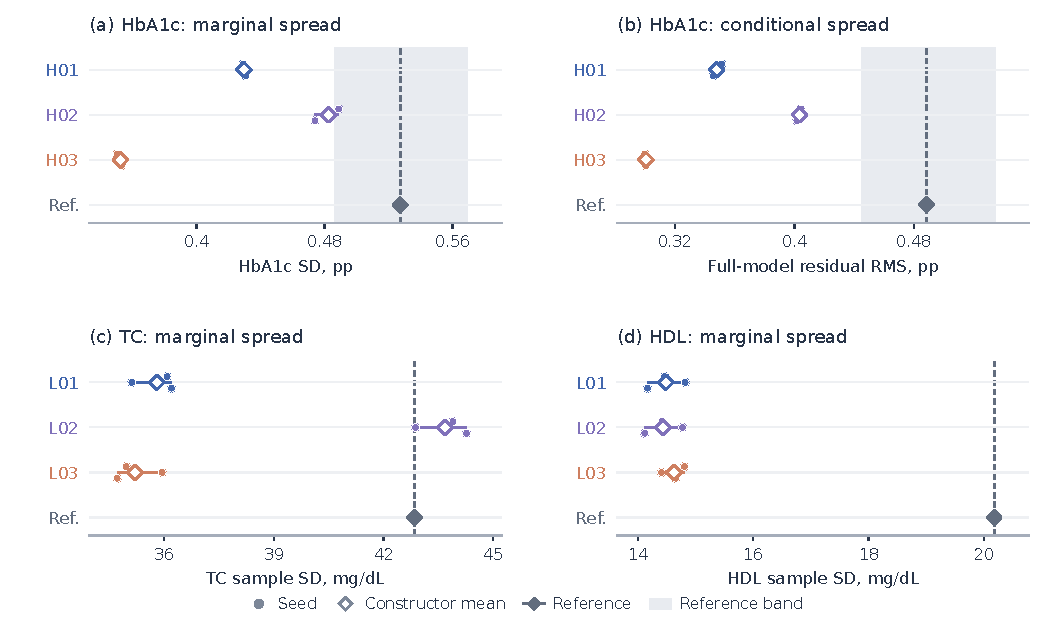
\includegraphics[width=\linewidth]{figures/figS3-dispersion.pdf}

\caption{Dispersion across all cross-task constructions. Panels show marginal HbA1c SD, HbA1c full-model residual RMS, and marginal TC and HDL SDs for each construction and its three final draws, retaining all 36 diagnostic values from the same 18 tables. HbA1c uses the population-SD diagnostic; lipids use sample SD. These quantities measure individual or residual spread, not uncertainty in a regression coefficient. H03's relatively close adjusted BMI effect in Figure 6 coexists with reduced HbA1c spread, and L02's close TC SD coexists with weak adjusted lipid dependence. Seed ranges reflect Monte Carlo variation conditional on the selected law. Gray HbA1c bands are empirical cluster-resampling stability bands; no reference interval is supplied for lipid SDs.}

\label{fig:8}

\end{figure}

The evaluation retained all 513 prespecified estimates and diagnostics, including the 54 primary outputs. Independent recomputation verified every value and all 324 matched reference comparisons; the maximum numerical difference was 5.33 × 10⁻¹⁴. The remaining 189 diagnostics lacked matching cached reference estimators and remained generated-only results. Across authors, eight original studies supplied 22 author–\allowbreak{}paper uses, including context/\allowbreak{}check-only uses; optional retrieval consumed seven query credits and one original download. All 132 declared source-check entries were unavailable under the implemented semantic rules because weighting or essential operator definitions were unresolved or unsupported (Table S6). Numerical source values still informed reviewed parameter derivations, but this batch provides neither measured numerical source-fit feedback nor a before/\allowbreak{}after revision benefit. The complete results and reviews retain every endpoint, unavailable comparison and implementation incident, including correction of the independent auditor's identifier parser without changing any generated table.


\FloatBarrier

\begingroup

\small

\renewcommand{\arraystretch}{1.22}

\begin{xltabular}{\linewidth}{@{}>{\hsize=1.350000\hsize\linewidth=\hsize\raggedright\arraybackslash}X>{\hsize=0.930000\hsize\linewidth=\hsize\raggedright\arraybackslash}X>{\hsize=0.930000\hsize\linewidth=\hsize\raggedright\arraybackslash}X>{\hsize=0.930000\hsize\linewidth=\hsize\raggedright\arraybackslash}X>{\hsize=0.930000\hsize\linewidth=\hsize\raggedright\arraybackslash}X>{\hsize=0.930000\hsize\linewidth=\hsize\raggedright\arraybackslash}X@{}}

\caption{Complete Q5 cross-task primary summaries. Each row summarizes three fixed final draws from one law. All 18 author–\allowbreak{}analysis combinations are retained. HbA1c entries are percentage points (pp); lipid slopes are mg/\allowbreak{}dL per 5 kg/\allowbreak{}m². Ranges are seed minima and maxima, not confidence intervals or evidence/\allowbreak{}model uncertainty.}\label{tab:10} \\

\toprule

\textbf{Request / analysis} & \textbf{Author} & \textbf{Units / increment} & \textbf{Reference} & \textbf{Generated mean} & \textbf{Seed min–\allowbreak{}max} \\

\midrule

\endfirsthead

\multicolumn{6}{l}{\small Table \thetable\ continued}\\

\toprule

\textbf{Request / analysis} & \textbf{Author} & \textbf{Units / increment} & \textbf{Reference} & \textbf{Generated mean} & \textbf{Seed min–\allowbreak{}max} \\

\midrule

\endhead

\bottomrule

\endfoot

HbA1c adjusted age & H01 & pp / 10 years & 0.075132 & 0.099545 & 0.094075–\allowbreak{}0.103606 \\

HbA1c BMI & H01 & pp / 5 kg/\allowbreak{}m² & 0.083643 & 0.060295 & 0.055769–\allowbreak{}0.063938 \\

HbA1c glucose-adjusted BMI & H01 & pp / 5 kg/\allowbreak{}m² & 0.056638 & 0.030469 & 0.027956–\allowbreak{}0.034291 \\

HbA1c adjusted age & H02 & pp / 10 years & 0.075132 & 0.099539 & 0.098162–\allowbreak{}0.100396 \\

HbA1c BMI & H02 & pp / 5 kg/\allowbreak{}m² & 0.083643 & 0.048923 & 0.029090–\allowbreak{}0.065499 \\

HbA1c glucose-adjusted BMI & H02 & pp / 5 kg/\allowbreak{}m² & 0.056638 & 0.019363 & 0.002308–\allowbreak{}0.030777 \\

HbA1c adjusted age & H03 & pp / 10 years & 0.075132 & 0.100912 & 0.096356–\allowbreak{}0.105015 \\

HbA1c BMI & H03 & pp / 5 kg/\allowbreak{}m² & 0.083643 & 0.056649 & 0.048449–\allowbreak{}0.063758 \\

HbA1c glucose-adjusted BMI & H03 & pp / 5 kg/\allowbreak{}m² & 0.056638 & 0.050978 & 0.044994–\allowbreak{}0.056901 \\

HDL BMI & L01 & mg/\allowbreak{}dL / 5 kg/\allowbreak{}m² & −4.623004 & −2.186526 & −2.286805–\allowbreak{}−2.118624 \\

TC BMI & L01 & mg/\allowbreak{}dL / 5 kg/\allowbreak{}m² & 5.683108 & 10.393977 & 9.992186–\allowbreak{}10.676486 \\

TC–\allowbreak{}HDL residual correlation & L01 & dimensionless & 0.512070 & 0.111234 & 0.108517–\allowbreak{}0.113140 \\

HDL BMI & L02 & mg/\allowbreak{}dL / 5 kg/\allowbreak{}m² & −4.623004 & −2.100390 & −2.194806–\allowbreak{}−2.035712 \\

TC BMI & L02 & mg/\allowbreak{}dL / 5 kg/\allowbreak{}m² & 5.683108 & 11.260864 & 10.811415–\allowbreak{}11.565687 \\

TC–\allowbreak{}HDL residual correlation & L02 & dimensionless & 0.512070 & 0.108283 & 0.105395–\allowbreak{}0.110194 \\

HDL BMI & L03 & mg/\allowbreak{}dL / 5 kg/\allowbreak{}m² & −4.623004 & −1.986781 & −2.122835–\allowbreak{}−1.913541 \\

TC BMI & L03 & mg/\allowbreak{}dL / 5 kg/\allowbreak{}m² & 5.683108 & 10.015112 & 8.617345–\allowbreak{}11.698752 \\

TC–\allowbreak{}HDL residual correlation & L03 & dimensionless & 0.512070 & 0.141343 & 0.121087–\allowbreak{}0.155368 \\

\end{xltabular}

\endgroup

HbA1c age adjusts for sex, BMI and glucose. HbA1c BMI adjusts for age/\allowbreak{}sex, with glucose added in the third analysis. Lipid BMI slopes adjust for age/\allowbreak{}sex; the residual correlation removes age/\allowbreak{}sex/\allowbreak{}BMI projections from both lipids on the same rows. H01–\allowbreak{}H03 belong only to this Q5 HbA1c request, and L01–\allowbreak{}L03 only to this Q5 lipid request; the L labels do not refer to the earlier Q2 literature arm. All 54 individual primary outputs and all 513 prespecified estimates/\allowbreak{}diagnostics remain in the complete endpoint table. The 324 matched reference comparisons and 189 generated-only diagnostics retain their original availability labels.


\FloatBarrier

\begingroup

\small

\renewcommand{\arraystretch}{1.22}

\begin{xltabular}{\linewidth}{@{}>{\raggedright\arraybackslash}X>{\raggedright\arraybackslash}X>{\raggedright\arraybackslash}X>{\raggedright\arraybackslash}X@{}}

\caption{Q5 original-source uses and unavailable feedback. Eight distinct originals supplied 22 author–\allowbreak{}paper uses, including context/\allowbreak{}check-only evidence. All six authors retained their initial laws. The 132 source-check entries were unavailable, not successful numerical comparisons or failed generators. The inventory counts the three lipid originals, with the Agongo correction [28] attached to its source rather than counted as a separate original study.}\label{tab:11} \\

\toprule

\textbf{Author} & \textbf{Original-source references} & \textbf{Paper uses} & \textbf{Unavailable source checks} \\

\midrule

\endfirsthead

\multicolumn{4}{l}{\small Table \thetable\ continued}\\

\toprule

\textbf{Author} & \textbf{Original-source references} & \textbf{Paper uses} & \textbf{Unavailable source checks} \\

\midrule

\endhead

\bottomrule

\endfoot

H01 & Pani [10]; Wisgerhof [14]; Skogberg [17]; Huang [21]; Ghazanfari [22] & 5 & 13 \\

H02 & Pani [10]; Skogberg [17]; Huang [21]; Ghazanfari [22] & 4 & 18 \\

H03 & Pani [10]; Skogberg [17]; Huang [21]; Ghazanfari [22] & 4 & 32 \\

L01 & Greiner [25]; Obirikorang [26]; Agongo [27,28] & 3 & 29 \\

L02 & Greiner [25]; Obirikorang [26]; Agongo [27,28] & 3 & 19 \\

L03 & Greiner [25]; Obirikorang [26]; Agongo [27,28] & 3 & 21 \\

Total & 8 distinct original studies & 22 & 132 \\

\end{xltabular}

\endgroup

The evidence-use inventory and source/\allowbreak{}code review retain the source IDs, numerical roles, unresolved definitions and actual retrieval activity. Unresolved weighting and unsupported or incompletely specified operators were not replaced with different statistics. Parameter derivations can therefore use reviewed source information while the corresponding runtime source comparison remains unavailable.


\clearpage

\subsection*{S6. Dependence sensitivity and the supporting construction}

The preceding open-search example acquired five seriously reviewed studies [9,10,12,13,14] without bibliographic seeds or desired signs. A fresh constructor selected a sex-stratified Gaussian copula with positive biomarker margins and generated one trial plus three complete 3,000-person tables. It retained the model after eleven approximate and 23 unavailable source comparisons per execution. Secondary BMI coefficients were 0.04217–\allowbreak{}0.05176 versus 0.05495 in the reused CHNS reference, secondary age was 0.01613–\allowbreak{}0.01771 versus 0.01530, and primary age was 0.00842–\allowbreak{}0.01084 versus 0.00811. Primary BMI/\allowbreak{}glucose were attenuated, and the female point direction and distributional tails remained imperfect. Supplementary Figure S3 retains all seven nonintercept effects and their uncertainty labels.


Before generating data or comparing targets, the source review identified an unreported BMI–\allowbreak{}glucose dependence. Two valid latent correlations, 0.10 and 0.40, implied conditional BMI coefficients of +0.03422 and −0.01095 while retaining the same margins, other bivariate laws and secondary projection. The delivered model used the declared assumption 0.25. This is an analytical sensitivity, not additional generated cohorts or a causal intervention. It demonstrates why an explicit data-generating law can identify which missing relationship matters to an intended use.


A separate analysis contextualized the same three tables with 100 community-disjoint resplits of the existing CHNS sample, drawing 3,000 people per side and retaining all 36 metrics. Secondary BMI and age discrepancies were on scales comparable with within-sample variation, while primary glucose/\allowbreak{}female and several joint/\allowbreak{}tail discrepancies were larger. The complete table preserves the nonexchangeable real-real and generated comparisons. These are descriptive interpretation aids, not a new population or retrospectively selected equivalence cutoff.


\begin{figure}[htbp]

\centering

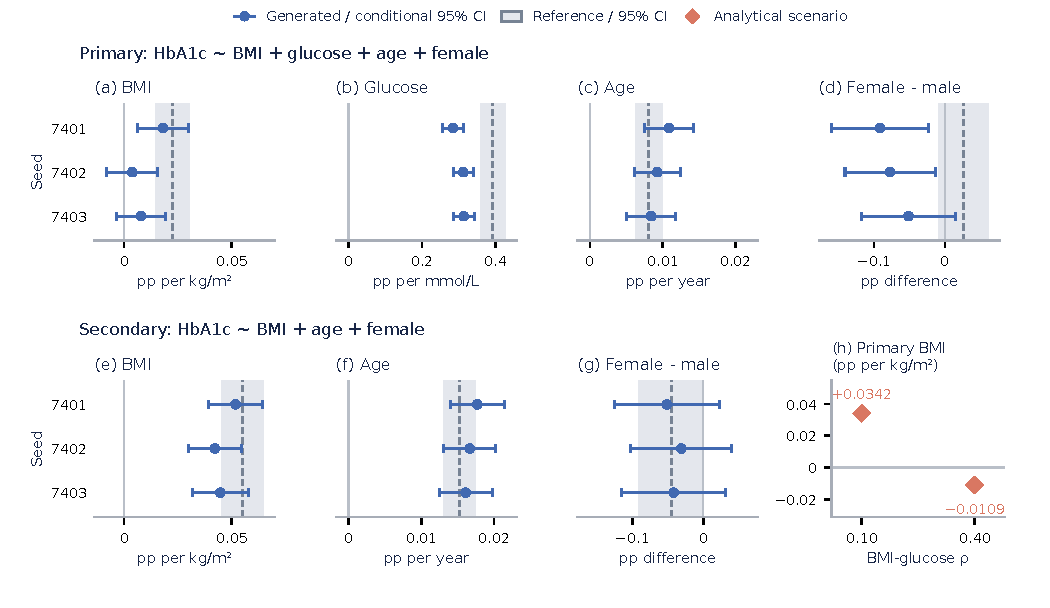
\includegraphics[width=\linewidth]{figures/figS4-analysis-use.pdf}

\caption{Analysis-specific usefulness and an unresolved joint dependence. Panels (a–\allowbreak{}d) show all primary-model nonintercept effects and (e–\allowbreak{}g) all secondary-model effects. Blue points are three fixed 3,000-person draws with conditional 95\% HC3-t intervals. Gray dashed lines and bands are exposed CHNS reference estimates and 95\% community-cluster CR1-t intervals; solid lines mark zero. All effects retain native units (pp: HbA1c percentage points), with shared limits for matching predictors. Generated intervals omit source, structural and transport uncertainty; overlap is not equivalence. Panel (h) displays two pre-generation analytical scenarios: latent BMI–\allowbreak{}glucose correlations 0.10 and 0.40 imply conditional BMI coefficients +0.03422 and −0.01095 while leaving marginal laws, other bivariate laws and the secondary projection unchanged. The delivered model used 0.25. These are not new draws, a fitted curve or a causal intervention. Retained initial/\allowbreak{}final stages alias the same three tables.}

\label{fig:9}

\end{figure}

The real-real context analysis reuses this evidence-to-generation law (\texttt{evcBuild01}, seeds 7401–\allowbreak{}7403). It does not evaluate the four Q4 authors. One hundred fixed community-disjoint partitions of the selected CHNS sample each provided two 3,000-person subsamples. Across the nine coefficients, 21 marginal summaries and six correlations, all 36 metrics were retained. Reduced-model BMI had median real-real difference 0.007239 versus generated-real symmetric discrepancy medians 0.004383–\allowbreak{}0.012727; reduced-model age had 0.001705 versus 0.001055–\allowbreak{}0.002387. Full-model glucose was 0.023839 versus 0.079642–\allowbreak{}0.109154. These selected examples illustrate agreement and disagreement relative to ordinary resampling variation; the complete report contains every metric. The resplits do not define population truth, independent cohorts or prespecified acceptable margins. The distances also have different geometry: real–\allowbreak{}real compares two complementary estimates, whereas the symmetric generated discrepancy averages distances from a fixed generated estimate to each. For illustrative estimates m+d and m−d and a generated estimate m, those distances are 2|d| and |d|. This identity is not an equality asserted for the fitted regressions; it explains why the comparison cannot itself supply an equivalence threshold.


\clearpage

\subsection*{S7. Prospective evaluation under the earlier method}

In HAALSI, eligible ages started at 40 years and the analysis used the released capillary point-of-care glucose measurement. Fasting was not an eligibility requirement. The fixed BMI and age contrasts were taken from the same additive glucose model with recorded sex. A second model estimated the difference in the BMI slope between women and men, adjusting for age. In Turkana, the two BMI slopes were adjusted for age and recorded sex. The correlation uses the residuals after adjusting both lipid measurements for age, sex and BMI.


Each case had five separately authored agent laws and one prespecified statistical generator (S01). The experiment produced 48 source-context and 36 target-context tables of 5,000 rows each. All authors retained their initial laws after source-only feedback. Initial and final labels therefore refer to the same 36 target tables. The public checkpoint preceding disclosure records work in progress. The final evaluation record documents the complete inventory, one reveal and independent recomputation of 6,704 checks. HAALSI had a prospectively withheld target. Turkana's exact estimates were withheld, with prior investigator exposure to adjacent findings. Later Q5 reused the same 397-person Turkana reference.


\FloatBarrier

\begingroup

\small

\renewcommand{\arraystretch}{1.22}

\begin{xltabular}{\linewidth}{@{}>{\hsize=1.350000\hsize\linewidth=\hsize\raggedright\arraybackslash}X>{\hsize=0.912500\hsize\linewidth=\hsize\raggedright\arraybackslash}X>{\hsize=0.912500\hsize\linewidth=\hsize\raggedright\arraybackslash}X>{\hsize=0.912500\hsize\linewidth=\hsize\raggedright\arraybackslash}X>{\hsize=0.912500\hsize\linewidth=\hsize\raggedright\arraybackslash}X@{}}

\caption{Six prespecified analyses under the earlier workflow. The columns report the measured-sample estimate, the minimum and maximum across 15 agent draws, the number agreeing in point sign, and the range of the three draws of the prescribed statistical law. The ranges describe draws under the candidate models. HAALSI glucose contrasts are in mmol/\allowbreak{}L, lipid slopes in mg/\allowbreak{}dL and the adjusted correlation is unitless.}\label{tab:12} \\

\toprule

\textbf{Analysis} & \textbf{Measured} & \textbf{Agent range} & \textbf{Same sign} & \textbf{S01 range} \\

\midrule

\endfirsthead

\multicolumn{5}{l}{\small Table \thetable\ continued}\\

\toprule

\textbf{Analysis} & \textbf{Measured} & \textbf{Agent range} & \textbf{Same sign} & \textbf{S01 range} \\

\midrule

\endhead

\bottomrule

\endfoot

HAALSI glucose, BMI per 5 kg/\allowbreak{}m² & 0.3138 & 0.3285 to 0.5698 & 15/\allowbreak{}15 & −0.0174 to 0.0180 \\

HAALSI glucose, age per 10 years & 0.2322 & 0.1136 to 0.3005 & 15/\allowbreak{}15 & −0.0170 to 0.0077 \\

HAALSI female-minus-male BMI slope per 5 kg/\allowbreak{}m² & −0.2440 & −0.2487 to 0.1903 & 8/\allowbreak{}15 & −0.0524 to 0.0046 \\

Turkana HDL, BMI per 5 kg/\allowbreak{}m² & −4.6230 & −3.5509 to −1.8173 & 15/\allowbreak{}15 & −0.1120 to 0.0710 \\

Turkana TC, BMI per 5 kg/\allowbreak{}m² & 5.6831 & 10.2822 to 15.0413 & 15/\allowbreak{}15 & −0.4657 to 0.0334 \\

Turkana residual TC–\allowbreak{}HDL correlation & 0.5121 & 0.1162 to 0.5361 & 15/\allowbreak{}15 & 0.3625 to 0.3840 \\

\end{xltabular}

\endgroup

\begin{figure}[htbp]

\centering

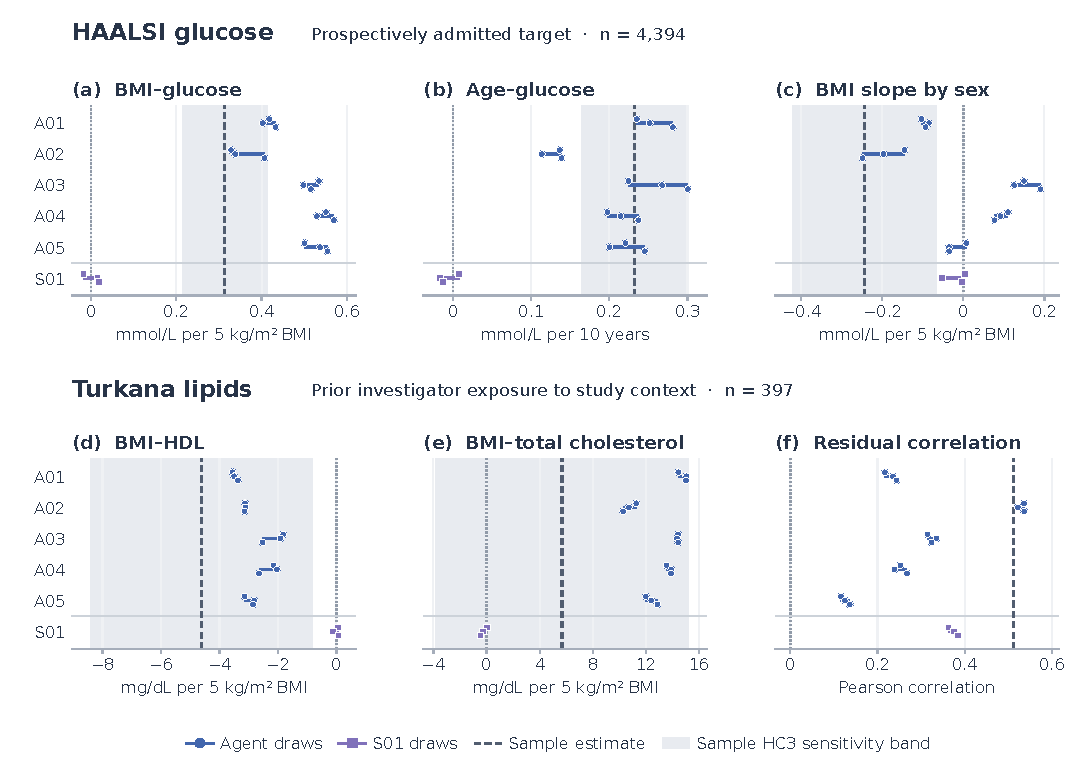
\includegraphics[width=\linewidth]{figures/figS5-prospective-wave.pdf}

\caption{Earlier prospective evaluation of whole-cohort generation. Blue circles show the three draws of each agent law and purple squares the three draws of the prescribed statistical law (S01). Short segments span draws. Dashed lines mark measured-sample estimates, and shaded bands give approximate 95\% HC3 sensitivity intervals for the five slopes. The residual correlation has no reference interval. HAALSI glucose main effects were directionally stable across agent draws. The sex difference in the BMI slope varied by construction. Turkana's total cholesterol point estimate had a reference interval that included zero. Its quantitative estimates were withheld before generation despite prior exposure to related published findings.}

\label{fig:10}

\end{figure}

The primary rule divided the absolute difference in each slope by the measured outcome's sample SD and used the absolute correlation difference directly. A construction passed when all nine comparisons (three analyses by three seeds) were at most 0.10. The agent counts at thresholds 0.05, 0.10, 0.20 and 0.30 were 1, 3, 5 and 5 of five for HAALSI and 0, 0, 1 and 4 for Turkana. Both S01 laws missed the primary criterion. For HAALSI, the discrepancies for three zero-valued effects were 0.0990, 0.0733 and 0.0770. The frozen decision closed the expansion. The prospective study predates the later interface for documenting numerical evidence use and supplies a separate evaluation of the underlying construction approach.


\begin{figure}[htbp]

\centering

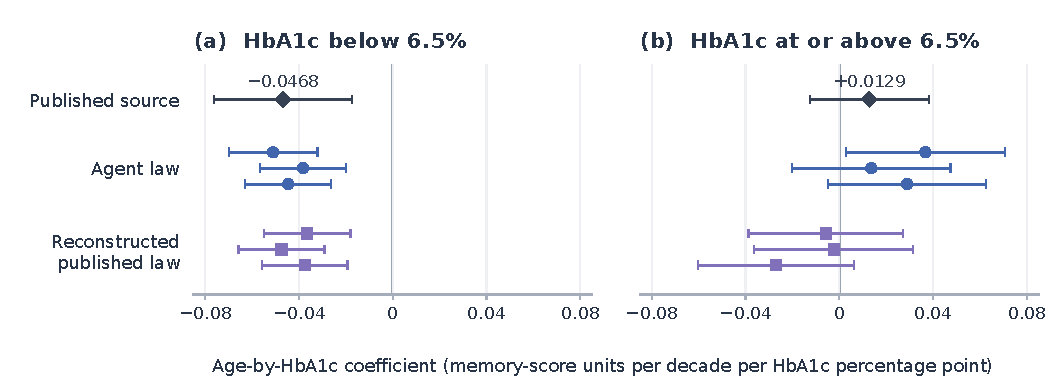
\includegraphics[width=\linewidth]{figures/fig2-hrs-comparison.pdf}

\caption{Two prespecified age–\allowbreak{}HbA1c interactions in a longitudinal memory model. Diamonds show the supplied coefficients; circles and squares show estimates from three draws per law (seeds 6101–\allowbreak{}6103, top to bottom). Bars show approximate 95\% Wald intervals calculated from the exported source standard errors or from the generated-table fits. Units are standardized memory-score change per decade per percentage point of HbA1c within the indicated branch. Each table contains 11,509 synthetic subjects and four visits per subject. The upper-branch signs differed between constructions. The six tables describe sampling under two frozen generating laws.}

\label{fig:11}

\end{figure}

\clearpage

\subsection*{S8. Full records and retained implementation incidents}

The \href{https://github.com/ziwang11112/evidence-guided-virtual-cohorts-2026}{public repository} provides original code, protocols, aggregate results and independent checks. The complete v0.9 extended record preserves all six original numerical tables and full methods/\allowbreak{}results. Its Table 2 supplies every main endpoint's adjustment set, units and reference interval; Tables 3–\allowbreak{}4 retain the main and summary-assisted values; Table 5 retains all latest seven effects; Table 6 retains the real-real comparison values. These archived tables preserve the earlier analyses alongside the separately sealed iron study.


The main study, summary-assisted study, statistical supplement, HRS example, preceding open-search construction, unified workflow replication and cross-task evidence-use study preserve separate frozen identities and complete endpoint outputs. The cross-task protocol, complete endpoint table, independent numerical review and scientific interpretation document the new unit. Earlier live A/\allowbreak{}B results, including the conditioned BMI mismatch and source-replay unavailability, remain in the extended record. Figure updates and added tables consume reviewed aggregates only; manuscript integration creates no cohorts or clinical fits. In the main study, seven authors inspected exploratory outputs and kept their laws, and thirteen finalized without exploration. The two earlier live authors both kept their models after the available review.


Individual real/\allowbreak{}generated tables, third-party originals and credentials remain local; clinical reruns require lawful access and the appropriate environment. Historical model identifiers and token costs are incompletely metered. Author/\allowbreak{}affiliation/\allowbreak{}funding/\allowbreak{}conflict/\allowbreak{}ethics/\allowbreak{}access/\allowbreak{}AI declarations and final submission formatting remain to be completed. No manuscript has been submitted.


The historical supplement retains earlier enrichment and direct-row construction, the divergent-moment repair, failed transport criteria, tail defects and revision trade-offs. The v0.16 reading draft preserves the earlier layout.


\subsection*{S9. Iron-status analysis and independent verification}

All six deliveries used two continuous columns, with three target analyses per delivery. The target survey comparison used the phlebotomy weight and 15 design degrees of freedom. Among 1,065 eligible positive-weight women, 979 had both measurements, 26 had hemoglobin only, 3 had ferritin only and 57 had neither. Thus 86 women were excluded from the paired analysis: 8.08\% of eligible records and 2.47\% of eligible phlebotomy-weight mass. Complete records represented 97.53\% of that weight mass. These percentages describe different denominators; the weighted percentage does not remove the need for a missingness assumption. The complete-case estimates characterize the observed-pair reference under the specified weights and design. Generalizing to all eligible women requires the unavailable pairs to be represented adequately by that analysis or another justified missing-data model; the existing phlebotomy weights alone do not establish this. No additional weighting adjustment or imputation for missing biomarker pairs was performed. A separate implementation reproduced all 21 point estimates (three reference, eighteen generated), the six target interval endpoints and the four unweighted cell counts. The study report gives all seed values and the evaluation protocol specifies the source replay, primary log-odds-ratio comparison and secondary analyses.


\subsection*{S10. Reproducing a program and tracing an agent decision}

In the iron task each fresh author received the same target description, source packet and clarification about a source summary. Only external source materials were allowed. The protocol specified numpy and pandas, a supplied random generator, the separate source and target contexts, and one source-only retain-or-revise opportunity. The task, evidence packet, A's final program and B's final program document the handoff. Run the programs with the recorded seeds and worker. The published code and aggregates support computational verification. Historical author-model snapshots and per-construction token counts are incompletely recorded, which limits reproduction of the original model-authoring sessions.


For the analytic part of Figure 5, let the four source counts be 173 (both low), 85 (low hemoglobin only), 331 (low ferritin only) and 1,082 (neither). Weight the first and third cells by two thirds and renormalize. Under A the final joint-low probability equals 0.8 times the reweighted joint-low probability plus 0.2 times the product of the two reweighted marginal probabilities. B keeps the original probabilities. This calculation describes the selected models and can be reproduced from published counts without sampling. The figure retains the original sealed deliveries and reference analysis alongside these model implications.


\subsection*{S11. A regression calculation used by one glycemia constructor}

This derivation belongs to CHNS Q1, arm E1, constructor A01, selected by ordinal identifier. Jansen et al. reported two age- and sex-adjusted regressions of HbA1c [9]. One used BMI as its predictor and the other used fasting glucose. The curated packet explicitly identified them as separate regressions. The constructor wanted to draw all three variables together. A slope from a regression on BMI alone can include part of the glucose association when BMI and glucose vary together, even after their age and sex terms are removed.


Let \(c_B\) and \(c_G\) be the two reported slopes. Let \(s_B\) and \(s_G\) be the residual standard deviations of BMI and glucose after accounting for age and sex, and let \(r\) be their residual correlation. The constructor assumed a linear HbA1c response to both residual predictors, with joint slopes \(\theta_B\) and \(\theta_G\) and an independent error. Projecting this response onto each predictor separately gives


\[
c_B = \theta_B + \theta_G r\,s_G/s_B
\]

\[
c_G = \theta_G + \theta_B r\,s_B/s_G
\]

The reported slopes were 0.13 mmol/\allowbreak{}mol per kg/\allowbreak{}m² of BMI and 2.29 mmol/\allowbreak{}mol per mmol/\allowbreak{}L of fasting glucose. A01 used residual standard deviations of 4.07611 kg/\allowbreak{}m² and 0.49694 mmol/\allowbreak{}L and assumed a residual correlation of 0.25. Solving for the joint slopes gave 0.0642173 and 2.1583154 in the respective IFCC response units. Multiplication by 0.09148 converted these slopes to 0.00587460 and 0.19744269 in HbA1c percentage-point units [11]. This construction recovers the two source projections under its own assumptions. The target model adds a separate glucose heterogeneity component. The source-to-model trace provides the response law, the source check and the ensuing target BMI discrepancy.


\subsection*{S12. Implementation of the system overview}

Each study uses a host coordinator to dispatch agent sessions and bind the research request to a dedicated execution path. Q4 describes the bounded open-retrieval workflow. Q5 provides a controller that binds the candidate files and a session runner that records trial feedback, decisions and closure. Its evaluator checks the closed state before reading pinned reference estimates.


In the iron study a case-specific adapter runs the agent's program with a source or target context using the isolated execution worker. The seal verifies the model and delivery hashes. The target analysis checks the sealed record before accessing the survey measurements. The execution notes document which checks were implemented in this adapter. The two studies share the separation of scientific authorship, numerical execution and evaluation, with different retrieval and feedback interfaces.


\clearpage

\subsection*{S13. Controlled check of joint-evidence construction}

We examined whether explicitly requesting joint consistency added value when the necessary evidence was already available. In one artificial four-variable population, both arms received the same 15 exact summaries: marginal means and SDs, the three predictor correlations, and four coefficients from two separately adjusted regressions. These summaries determine the requested joint linear projection and residual variance, but not the full probability distribution. Two fresh constructors per arm wrote their own programs without target coefficients, a supplied solver or earlier results. The additional-instruction arm was asked to reconcile all constraints jointly and separate explained from residual variation; the ordinary arm received the same scientific task and evidence. The protocol, evaluation rules and all four programs were frozen before sampling. Each program generated three 10,000-row tables using the fixed seeds 8101–\allowbreak{}8103; no trial or feedback revision was allowed.


All four authors selected the same Gaussian law and recovered the implied joint coefficients 0.25, 0.65 and −0.40 and residual variance 0.6775. All twelve attempts succeeded. O1/\allowbreak{}C2 and O2/\allowbreak{}C1 used matching RNG layouts, so corresponding same-seed outputs were identical: twelve deliveries represented six distinct tables and one law. The three seeds within each layout gave distinct tables. In both arms, mean absolute standardized joint-coefficient errors were 0.01244, 0.01024 and 0.01337; mean absolute log residual-SD error was 0.00613. Metrics were averaged over seeds within constructors and then equally across the two constructors, without pooled-row inference.


The ordinary construction already performed the required statistical reconciliation. This bounded diagnostic therefore supplied no evidence for adding the extra instruction. It is not biomedical validation or a test of uncertain extraction, heterogeneous populations, tail behavior or feedback. The target coefficients were withheld from authors but algebraically implied by the supplied summaries; their recovery does not demonstrate learning an unconstrained relationship. The complete report retains all runs, failure checks, duplicate-output accounting and separate implementation/\allowbreak{}results audits. No additional cases or constructions were added after these results.


\subsection*{S14. Historical synthetic training on a later real sample}

The October 25 temporal pilot tested a different input setting and direct-row output route. Two fresh authors literally supplied 128-row cohorts from rich outcome-by-sex-conditioned summaries of 128 real NHANES2015–\allowbreak{}16 training participants. Inputs included counts, means, SDs, quantiles and regularized Gaussian-rank correlations. An ordinary Gaussian-copula generator supplied 100 comparison cohorts. The predictor set was age, sex, BMI, waist and systolic blood pressure; HbA1c and design variables were not predictors. The outcome was current HbA1c at least 5.7\% among adults with BMI at least 30, not future diabetes or obesity classification.


All preprocessing and classifier artifacts were locked before the NHANES2017–\allowbreak{}18 test download. Evaluation used 1,811 eligible test participants. Table S8 retains the primary logistic and secondary histogram-gradient-boosting results. A prevalence-only predictor using the training prevalence 68/\allowbreak{}128 had AUC 0.5 and Brier score 0.248578. Both Agent cohorts carried predictive information, but neither exceeded the real-training AUC. One was below and one above the ordinary-generation median in each classifier, both within the ordinary draw distributions. The ordinary median summarizes 100 draws, not 100 independent studies. Neither a confidence interval nor a noninferiority test was calculated for the AUC differences. The complete report also retains log loss, balanced accuracy and weighted sensitivity analyses. This is evidence of historical downstream utility under rich real-training summaries, not a literature-only or current-controller confirmation.


\FloatBarrier

\begingroup

\small

\renewcommand{\arraystretch}{1.22}

\begin{xltabular}{\linewidth}{@{}>{\raggedright\arraybackslash}X>{\raggedright\arraybackslash}X>{\raggedright\arraybackslash}X>{\raggedright\arraybackslash}X@{}}

\caption{Historical synthetic-training utility on later real participants. Higher AUC and lower Brier score indicate better performance on this selected sample. Agent rows come from two literal 128-row datasets. The ordinary entry is the median across 100 generated training cohorts. Both classifiers used the same 1,811-person test; no rows were regenerated after test disclosure.}\label{tab:13} \\

\toprule

\textbf{Classifier} & \textbf{Training cohort} & \textbf{AUC} & \textbf{Brier score} \\

\midrule

\endfirsthead

\multicolumn{4}{l}{\small Table \thetable\ continued}\\

\toprule

\textbf{Classifier} & \textbf{Training cohort} & \textbf{AUC} & \textbf{Brier score} \\

\midrule

\endhead

\bottomrule

\endfoot

Logistic (primary) & Real 128 & 0.734936 & 0.210303 \\

Logistic (primary) & Agent A1 & 0.712130 & 0.216229 \\

Logistic (primary) & Agent A2 & 0.726871 & 0.213445 \\

Logistic (primary) & Ordinary, median & 0.717394 & 0.215560 \\

Histogram boosting (secondary) & Real 128 & 0.660930 & 0.240598 \\

Histogram boosting (secondary) & Agent A1 & 0.634484 & 0.247879 \\

Histogram boosting (secondary) & Agent A2 & 0.646883 & 0.242525 \\

Histogram boosting (secondary) & Ordinary, median & 0.638858 & 0.261487 \\

\end{xltabular}

\endgroup

\subsection*{S15. Later adaptive and source-context implementation}

The bounded adaptive case executed 28 dispatched actions, including retrieval, construction, inspection and a final choice. The author produced two scientific models and six tables, then retained the initial model. Its sensitivity altered two analyses in different directions of reference agreement. This is executed scientific decision-making, with zero initial-to-selected-final improvement. It is not a new clinical population or a controlled estimate of a feedback benefit.


The source-conditioned replay next linked one Agent-authored shared source/\allowbreak{}target law to eight sex/\allowbreak{}site-stratified BMI–\allowbreak{}lipid coefficients from the \href{https://doi.org/10.1136/bmjgh-2019-001542}{admitted source study}. Four source contexts and three seeds yielded twelve 8,000-row source tables and 24 numerical projections. All reported directions were retained, with independent QR/\allowbreak{}FWL arithmetic agreement within 5.9e-15. The source weighting and BMI-standardization convention remained unresolved: every strict semantic check stayed unavailable, and the numerical projections were explicitly assumption-dependent. The Agent retained the initial law. Three subsequent 3,000-row target-scenario tables supported nine requested estimates and 69 descriptive calculations without a new clinical-reference comparison. Residual component coupling could change substantially while the mean slopes remained fixed. These results demonstrate source-conditioned execution and attributable assumptions, not independently established target accuracy.


The method-coverage audit separates these implementations from the curated Q1 comparison, open-retrieval Q4 workflow, Q5 evidence-use interface, iron source pilot, HRS reconstruction and earlier prospective controller. They share the scientific procedure described in Sections 2–\allowbreak{}3. Optional later components were not exercised in every historical case and are not credited retroactively. No participant or generated row table was opened for this manuscript integration.


\clearpage

\subsection*{S16. Reference populations and estimands}

\FloatBarrier

\begingroup

\small

\renewcommand{\arraystretch}{1.22}

\begin{xltabular}{\linewidth}{@{}>{\raggedright\arraybackslash}X>{\raggedright\arraybackslash}X>{\raggedright\arraybackslash}X>{\raggedright\arraybackslash}X@{}}

\caption{Reference definitions, analytical populations and uncertainty. Sample sizes are measured-reference counts except in HRS, where the comparison uses supplied model exports and the stated count describes each generated table. HbA1c effects are in percentage points (pp). Reference intervals and stability bands describe different sources of uncertainty; none is an equivalence margin or an interval for source-to-target transfer error.}\label{tab:14} \\

\toprule

\textbf{Reference and study use} & \textbf{Eligibility and size} & \textbf{Weighting and scientific estimand} & \textbf{Uncertainty and reference status} \\

\midrule

\endfirsthead

\multicolumn{4}{l}{\small Table \thetable\ continued}\\

\toprule

\textbf{Reference and study use} & \textbf{Eligibility and size} & \textbf{Weighting and scientific estimand} & \textbf{Uncertainty and reference status} \\

\midrule

\endhead

\bottomrule

\endfoot

CHNS 2009: Q1, Q2, Q4 and preceding CHNS analyses & 6,631 linked adults aged 35–\allowbreak{}74 in 218 communities, complete for recorded age, sex, BMI, central glucose and HbA1c. BMI uses finite positive height and weight; a height/\allowbreak{}weight cleaning flag of 9 makes that measurement unavailable. No diabetes, treatment or pregnancy exclusion; individual fasting adherence was not verified. & Unweighted selected-sample regressions. The Q1/\allowbreak{}Q4 focal coefficients are BMI adjusted for age/\allowbreak{}sex, glucose adjusted for age/\allowbreak{}sex, and age adjusted for sex/\allowbreak{}BMI/\allowbreak{}glucose; units are HbA1c pp per kg/\allowbreak{}m², mmol/\allowbreak{}L and year, respectively. Q2 additionally evaluates supplied correlations. & Regression reference intervals use the community-cluster CR1 sandwich and a t cutoff with 217 degrees of freedom. These are not national survey estimates. The project references had been exposed before Q1/\allowbreak{}Q2/\allowbreak{}Q4; Q2 deliberately supplied target summaries. \\

ENSANUT 2018: Q1, Q4 and Q5 glycemia & 6,931 adults aged 25–\allowbreak{}79 with concordant laboratory/\allowbreak{}anthropometry age and sex; no reported prior doctor diagnosis of diabetes/\allowbreak{}high blood sugar; recorded 8–\allowbreak{}12-hour fast; finite positive serum glucose below 126 mg/\allowbreak{}dL and positive HbA1c; eligible standing anthropometry and questionnaire-routed pregnancy/\allowbreak{}lactation status, detailed below. No verified medication or anemia exclusion. & Each sex-by-age cell has mass 1/\allowbreak{}8: recorded male/\allowbreak{}female crossed with 25–\allowbreak{}39, 40–\allowbreak{}54, 55–\allowbreak{}69 and 70–\allowbreak{}79 years. A reference participant in cell h has weight 1/(8n\_h). HbA1c regressions estimate age per 10 years adjusted for sex/\allowbreak{}BMI/\allowbreak{}glucose, and BMI per 5 kg/\allowbreak{}m² adjusted for age/\allowbreak{}sex with or without glucose. This is an equal-cell analytical standard, not national survey weighting. & Empirical 2.5th–\allowbreak{}97.5th percentile stability bands from 399 fixed cluster-resampling attempts using laboratory strata/\allowbreak{}PSUs and recomputed cell weights; all 399 were valid. These bands have no claimed national confidence coverage. The reference was previously exposed at project level. \\

NHANES August 2021–\allowbreak{}August 2023: iron & 979 women aged 20–\allowbreak{}44 with confirmed nonpregnant status (RIDEXPRG=2), positive phlebotomy weight and both hemoglobin and raw ferritin, among 1,065 otherwise eligible positive-weight women. Missing pairs excluded 86 women, representing 2.47\% of eligible weight mass; no additional item-nonresponse adjustment or imputation. No CRP requirement. & WTPH2YR-weighted complete-case crude odds ratio for hemoglobin <12 g/\allowbreak{}dL by ferritin <15 µg/\allowbreak{}L (primary comparison on log OR), joint-low prevalence and weighted Spearman correlation using midranks. The release's detection-limit convention is retained. & Stratified delete-one-PSU jackknife, 15 strata, 30 PSUs and 15 design degrees of freedom; t intervals on log-OR, logit-prevalence and Fisher-z correlation scales, back-transformed. Protocol and deliveries preceded target biomarker access; NHANES was already known to the project. Inference concerns the observed-pair reference under this design. \\

HAALSI baseline v3.0: earlier prospective wave & 4,394 adults aged ≥40, with recognized recorded sex and finite age, positive cleaned BMI and positive cleaned capillary point-of-care glucose. Age is census age at 31 July 2014 sample selection. No fasting or treatment restriction, imputation, flag-based trimming or winsorization; finite positive released boundary values are retained. & Unweighted selected-sample glucose regressions: BMI per 5 kg/\allowbreak{}m² adjusted for age/\allowbreak{}sex; age per 10 years adjusted for BMI/\allowbreak{}sex; female-minus-male difference in the BMI slope from a model also adjusting for age. Outcome units are mmol/\allowbreak{}L. & Reference-only HC3 normal working sensitivity intervals; no survey-design, cluster or transport coverage claim. Exact target results were prospectively withheld from construction. The outcome is the released cleaned measurement, without assuming equivalence to a fasting serum/\allowbreak{}plasma assay. \\

Turkana/\allowbreak{}Laikipia 2018–\allowbreak{}2019 study context: earlier prospective wave and Q5 lipids & 397 adults aged ≥18 with recorded sex F/\allowbreak{}M, finite age and positive finite BMI, total cholesterol and HDL cholesterol. No additional disease, pregnancy, fasting, lifestyle, outlier or TC≥HDL exclusion. Lipids were recorded in mg/\allowbreak{}dL; generated mmol/\allowbreak{}L values were converted with the frozen factor 38.67. & Unweighted age/\allowbreak{}sex-adjusted BMI slopes for TC and HDL, in mg/\allowbreak{}dL per 5 kg/\allowbreak{}m², and Pearson correlation of their residuals after age/\allowbreak{}sex/\allowbreak{}BMI adjustment on the same rows. The pooled site/\allowbreak{}lifestyle composition is that of the selected sample. & HC3 normal assumption-conditional sensitivity intervals for slopes; no interval supplied for residual correlation. Sampling weights and cluster identifiers were not supplied. Earlier exact estimates were withheld despite prior investigator exposure to related findings; Q5 reused this exposed reference. \\

HRS published recipient-stage example: Q3 & Supplied-model reconstruction, with no new selection or analysis of HRS participants. Each generated table has 11,509 synthetic subjects and four visits at 0, 2, 4 and 6 years (46,036 rows), using exported demographic cells. The output contract permits baseline ages 50–\allowbreak{}100, female/\allowbreak{}male sex and white/\allowbreak{}black race; these are generation definitions, not a newly verified source-cohort eligibility rule. & The supplied mixed model has subject intercepts/\allowbreak{}slopes, age centered at 60 and scaled per decade, piecewise HbA1c terms below/\allowbreak{}above 6.5\%, and the source covariates/\allowbreak{}interactions. Focal interactions measure standardized-memory-score change per decade per HbA1c pp within each branch. & Approximate Wald intervals use exported source SEs or generated-table fits. Source coefficients are legitimate inputs. The published observed analysis had 43,500 visits, whereas generated schedules are balanced; equal precision is not assumed. This is source-model reconstruction, not a withheld-patient validation or national HRS inference. \\

\end{xltabular}

\endgroup

\textbf{ENSANUT measurement restrictions.} Laboratory diagnosis response P7 must equal 2; prior, pregnancy-related, unknown or missing diagnosis responses are excluded. For women aged 25–\allowbreak{}49, anthropometry P6 must equal 4 (neither pregnant nor breastfeeding); unasked groups are not assigned negative responses. BMI uses the first complete admissible same-ordinal weight/\allowbreak{}standing-height pair, or the second only when the first is unavailable. Weight 222.222 kg and height 222.2 cm are treated as documented nonmeasurement codes in both repeats. Both age-routed measurement-block result flags must equal 1 (“no problem”); at age ≥60, the documented standing route must be P11=1 or 4. Explicit not-weighed or alternative-route documentation, including contradictions with usable standing values, is excluded uniformly. These are investigator-defined measurement/\allowbreak{}documentation restrictions, not proof that excluded numeric readings are erroneous. There is no cross-repeat mixing, alternative-stature reconstruction, imputation or distribution-based trimming. Serum glucose remains in mg/\allowbreak{}dL and HbA1c in percentage points for analysis; external plasma-glucose evidence requires a specimen/\allowbreak{}assay transfer assumption.


All reference definitions retain their original study-specific role. A valid numerical comparison does not by itself establish population transport, causal interpretation or calibrated inference from synthetic rows.


\clearpage

\subsection*{S17. Authoring and reproducibility conditions}

\FloatBarrier

\begingroup

\small

\renewcommand{\arraystretch}{1.22}

\begin{xltabular}{\linewidth}{@{}>{\raggedright\arraybackslash}X>{\raggedright\arraybackslash}X>{\raggedright\arraybackslash}X>{\raggedright\arraybackslash}X@{}}

\caption{Implementation records for the principal construction studies. Each controller manages a study-specific execution process around externally dispatched authors; it does not provide a reproducibly specified model-service invocation.}\label{tab:15} \\

\toprule

\textbf{Study and authors} & \textbf{Recorded model identity} & \textbf{Evidence and required review} & \textbf{Trial budget and executed decisions} \\

\midrule

\endfirsthead

\multicolumn{4}{l}{\small Table \thetable\ continued}\\

\toprule

\textbf{Study and authors} & \textbf{Recorded model identity} & \textbf{Evidence and required review} & \textbf{Trial budget and executed decisions} \\

\midrule

\endhead

\bottomrule

\endfoot

Q1: 20 Agent authors; 4 prescribed constructions & Dispatches record an inherited host model; exact backend and token costs unavailable. & Curated condition-specific packets; no retrieval. Separate reviewers checked numerical uptake and finite moments before final selection. Source calculations were analytic, without simulated source populations. & At most two exploratory attempts, one scientific revision and three final draws per construction; 3,000 rows per draw. Seven authors inspected a trial and retained; thirteen finalized without exploration. All 72 final tables followed common closure. \\

Q4: 4 Agent authors & Fresh context IDs and timestamps retained; exact backend/\allowbreak{}inference configuration not specified. & Up to eight query credits, including fetch metadata, and four originals per author. Source/\allowbreak{}proposal review preceded implementation; up to two source/\allowbreak{}mechanical review rounds per stage. Independent review required before freeze and final selection. & One initial and at most one revised trial; three final draws, each 3,000 rows. All four retained the first frozen law. Generated diagnostics included qualified source comparisons, without source-population replay. Twelve unchanged final tables were analyzed by the corrected evaluator. \\

Q5: 6 Agent authors & Shared model service and external author IDs recorded; exact backend/\allowbreak{}inference configuration not specified. & Reviewed packets; optional four query credits and two new originals per author before freeze. Source/\allowbreak{}proposal, candidate and final-decision reviews required. & One initial and one optional revised/\allowbreak{}repair trial, sharing the second slot; three final draws, each 3,000 rows. All retained. All 132 source comparisons were unavailable; generated diagnostics and reviewed derivations remained available. Reference reading followed six closures. \\

Iron: 2 Agent authors & Candidate stages and hashes retained; exact author-model snapshot/\allowbreak{}inference configuration not recorded in admission files. & Shared packet and pre-author source clarification. Host source-only review and hash locks; the compact adapter did not implement Q4/\allowbreak{}Q5 review-state gates. & One initial source review and one retain/\allowbreak{}revise opportunity; 100,000 rows at seed 4101 per source run. A repaired its upper tail and repeated the source check; B retained. Three 5,000-row final tables per law at seeds 5101–\allowbreak{}5103 were sealed before target biomarker access. \\

\end{xltabular}

\endgroup

Fresh-context instructions restricted author inputs procedurally; the sampling program ran in a network-disabled isolated worker. Exact model snapshots, inference settings and per-construction token usage are incompletely recorded. These omissions limit reconstruction of the original authoring sessions, separately from inspecting and replaying the frozen statistical programs.


The reproducibility guide distinguishes aggregate-display regeneration, frozen-program replay and clinical-reference evaluation. Its iron example documents the existing isolated interface and numerical environment as an unexecuted reference recipe, not a verified clean-install reproduction. Complete original Agent sessions cannot be reconstructed from the incomplete or unpublished model and conversation records.


In Q4 the host/\allowbreak{}root Agent performed source and static reviews; Q5 also used separately dispatched review Agents, with final decisions reviewed by the root coordinator. A distinct review role does not imply a different model family or a reviewer unexposed to earlier project results. The Q4 record distinguishes source-transcription corrections, such as two printed residual variances, from a mechanical path-name repair and from a post-trial change of scientific law.

\end{document}
